\documentclass{article}
\usepackage[utf8]{inputenc}
\usepackage[spanish]{babel}

\title{BAD: Autenticación mediante la utilización de señales EMG}

\author{
    Bezdjian Alejandro (Leg. Nº 52108) \\
    \and
    Marzoratti, Luis (Leg. Nº 54449)
}
\date{Julio 2018}

\usepackage{subfigure}
\usepackage{graphicx}
\usepackage{amsmath}
\usepackage{mathtools}
\usepackage[normalem]{ulem}
\DeclarePairedDelimiter\abs{\lvert}{\rvert}%
\usepackage{minted}
\usepackage[a4paper, total={6in, 8in}]{geometry}
\usepackage[
backend=biber,
style=alphabetic,
sorting=ynt
]{biblatex}
\addbibresource{references.bib}

\begin{document}

\maketitle
\thispagestyle{empty}
\clearpage
\tableofcontents
\clearpage

\section{Abstract}

\paragraph{
La autenticación multifactor combina credenciales de distinto tipo para crear una defensa por capas y prevenir accesos no autorizados. En este trabajo proponemos un sistema que provee autenticación multifactor utilizando ``algo que tengo'' y ``algo que soy'' mediante un dispositivo de autenticación biométrica que requiere de una participación activa del usuario. Está participación permite solucionar un problema intrínseco de los sistemas biométricos que es no poder cambiar una clave que depende de una característica propia del individuo como lo es una huella digital.
}
\paragraph{
Para realizar esto llevamos a cabo una comparación de distintos dispositivos biométricos de bajo costo para el desarrollo de aplicaciones de IoT. Se analizaron los dispositivos True Sense, Olimex EEG/EMG Shield y Muse Headband buscando ventajas y problemas para su utilización en una aplicación de IoT. Realizamos experimentos y obtuvimos datos para poder determinar que dispositivo y que tipo de señal era más apropiada para nuestro propósito.
}
\paragraph{
El sistema propuesto está orientado a proveer un servicio a empresas que ya utilicen autenticación mediante una contraseña y busquen aumentar su nivel de seguridad. Implementamos una API genérica, denominada BAD API (Biosignal Authentication Device) que permite utilizar dispositivos biométricos para proveer una autenticación multifactor como servicio. Para mostrar su funcionamiento desarrollamos un dispositivo prototipo que codifica una señal de EMG (electromiografía) generada activamente por el usuario en una contraseña binaria y desarrollamos una aplicación web de prueba que consume el servicio.
}

\section{Introducción}
\paragraph{
En la actualidad, internet se ha vuelto una herramienta fundamental en casi todos los aspectos del ser ser humano. Hace ya mucho tiempo que dejó de ser tan solo un método de comunicación conveniente. Por ejemplo, las personas ahorran mucho tiempo y dinero comprando en sitios e-commerce o haciendo trámites online. También, se entretienen con juegos, plataformas de música y video y con las redes sociales. Sin embargo, la mayoría de sitios web siguen requiriendo a los usuarios que se registren utilizando un nombre de usuario y una contraseña, un método que sigue sobreviviendo desde el comienzo de internet \cite{internet}.
}
\paragraph{
 No todos los sitios de internet toman los recaudos necesarios en materia de seguridad para almacenar las contraseñas o para no permitir que atacantes intenten adivinar las mismas. Esto puede suceder por desconocimiento o porque los sistemas quedan desactualizados y sin mantenimiento o por vulnerabilidades de seguridad, entre otros.
}
\paragraph{
Otro de los problemas los usuarios por lo general suelen olvidar las contraseñas muy largas y complejas (lo que hace que las contraseñas sean más seguras). Para contrarrestar este último punto, muchos sitios obligan a las personas a generar contraseñas que contengan letras mayúsculas y/o símbolos, esto sirve para aumentar la cantidad total de posibles contraseñas, y así disminuir la posibilidad de éxito frente a un ataque. Si bien esto mejora la seguridad frente a una búsqueda aleatoria o por fuerza bruta, los atacantes realizan búsquedas más inteligentes utilizando contraseñas o palabras conocidas, transformaciones simples de las mismas y también información de los usuarios (si la tienen).
}
\paragraph{
Para empeorar aún más la situación, los usuarios suelen repetir contraseñas entre los diferentes sitios para no olvidarlas, lo que hace que exista una fuga de información indirecta cuando un sitio web es hackeado. Actualmente se sabe que más de cinco mil millones de contraseñas fueron adquiridas por hackeos públicamente conocidos \cite{haveibeenpwned}. Es por esto que los sistemas seguros modernos suelen no utilizar únicamente una contraseña para autenticar a un usuario.
}
\paragraph{
Mejorar la seguridad en internet y proteger la información de los usuarios es sumamente importante y para eso los esquemas de autenticación multifactor pueden proveer una mejora a los esquemas actuales.
}
\paragraph{
El cuerpo humano posee una actividad eléctrica natural que puede utilizarse para transmitir información a un dispositivo electrónico. Con este objetivo, son de particular importancia la electromiografía y la electroencefalografía. En el pasado estas señales eran utilizadas únicamente para propósitos médicos, pero en los últimos años con el surgimiento de las Brain Computer Interfaces (BCI) aumentó la disponibilidad de dispositivos de uso comercial. A la vez con la surgimiento de dispositivos \textit{wearables} aparecieron nuevas posibilidades para la aplicación de sensores biométricos. Las aplicaciones de ésta tecnología son muy variadas, van desde control de prótesis robóticas \cite{veer2015} hasta otras más tradicionales como el registro de actividad cerebral durante el sueño o meditación \cite{kaur2015}.
}
\paragraph{
Uno de los aspectos más interesantes de este tipo de señales es que, si se logran los avances tecnológicos necesarios, podría suceder que los usuarios no necesiten realizar una acción extra para usar estas señales en la autenticación de un sistema, ya que podrían obtenerse a través de dispositivos que usa habitualmente de forma automática, logrando una mejor experiencia de usuario.
}
\section{Justificación del trabajo}
\paragraph{
En este trabajo se evaluará la factibilidad de la utilización de señales EMG o EEG para utilizar como método de autenticación o segundo factor. Es por eso que se investigará si existe información intrínseca de los individuos en dichas señales y de qué manera se pueden implementar para que utilizarlo en sistemas existentes sea lo más simple posible.
}
\paragraph{
Este tipo de señales tienen las ventajas que se obtienen mediante métodos no invasivos y con una participación tanto pasiva como activa de los individuos, lo que ofrece flexibilidad para aumentaría la aceptación psicológica de los mismos.
}
\paragraph{
En primer lugar evaluamos distintos dispositivos de EMG y EEG disponibles para su uso en un sistema de autenticación. Esto implicó implementar una interfaz para comunicarse con los mismos y poder determinar las ventajas y desventajas de cada uno. A partir de estos datos tomamos la decisión de quedarnos con uno para diseñar una implementación testigo en la que se pueda observar la factibilidad del sistema, finalmente presentamos una API para dar un uso comercial al mismo
}
\paragraph{
Nuestro trabajo de divide en tres partes: primero se presentan los distintos tipos de señales biométricas disponibles y el estado del arte en su uso como factor de autenticación. Luego se comparan distintos dispositivos biométricos con el fin de decidir cual utilizar para una implementación y habiendo elegido uno se detalla el procesamiento de la señal obtenida. Para finalizar se presenta una implementación de una API genérica para realizar autenticación mediante una señal biométrica con un fin comercial.
}

\section{Estado del arte}
\subsection{Electromiografía (EMG)}
\paragraph{
EMG es una técnica de electro diagnóstico médico para grabar la actividad eléctrica de los músculos esqueléticos (unidos al esqueleto) provenientes del sistema nervioso. Existen dos tipos de EMG superficial e intramuscular. EMG superficial consiste en colocar electrodos, pequeños discos metálicos de algún material altamente conductivo, sobre la piel. Generalmente se aplica alguna sustancia entre el electrodo y la piel para reducir la impedancia entre ellos, como por ejemplo alcohol. Este tipo de EMG permite una visión general del funcionamiento del músculo y tienen la ventaja de ser procedimientos no invasivos. En EMG intramuscular los electrodos son agujas que se insertan en la piel hasta el tejido muscular, esto permite un análisis más detallado (debido, principalmente, a la reducción de ruido en las señales) de la actividad en el músculo pero tiene la desventaja de ser invasivo.
}
\paragraph{
Cuando se observan biopotenciales colocando electrodos sobre la piel, no se registran potenciales intracelulares sino potenciales extracelulares, que son la manifestación de los primeros en el exterior al imprimir
corrientes sobre los tejidos circundantes, que ofician de conductor de volumen. Además, generalmente no se observan potenciales de acción individuales, sino la superposición de un gran número de éstos originados en distintas células, que se combinan en el mencionado conductor de volumen. La amplitud y la morfología de las señales observadas dependen de múltiples factores, como el tipo de células involucradas, la cantidad de ellas y la distancia a la superficie, entre otras. \cite{haberman2016}
}
\paragraph{
Para este proyecto se consideraron únicamente dispositivos de EMG superficial.
}

\subsection{Electroencefalografía (EEG)}
\paragraph{
EEG es otra técnica de electro diagnóstico médico que sirve para grabar la actividad eléctrica del cerebro. Así como con EMG puede o no ser invasiva dependiendo del nivel de detalle requerido. Las técnicas no invasivas son más frecuentes, ya que las invasivas requieren perforaciones en el cráneo por lo que son utilizadas en pacientes con condiciones severas. Existen aplicaciones comerciales de EEG superficial para el monitoreo del sueño y meditación como el Muse Headband [Figura \ref{fig:muse}]. Las señales de EEG son difíciles de asociar a patrones cognitivos debido a la complejidad del cerebro humano.
}
\paragraph{
En general, debido a que las mediciones se realizan con electrodos en el cuero cabelludo, difícilmente se puedan obtener buenas mediciones de la actividad directa del Sistema Nervioso Central y son fuertemente dependientes de la ubicación de los electrodos. Además, si bien es posible detectar de manera general las áreas del cerebro que se encuentran en actividad, la localización espacial es bastante pobre y es muy difícil asociar que acciones específicas producen las señales.
}
\paragraph{
Otro aspecto importante es que los dispositivos con mejor resolución son muy costosos, siendo principalmente utilizados en aplicaciones médicas. Los dispositivos comerciales sacrifican resolución y/o calidad de señal para poder disminuir el costo. En el caso del Muse Headband, está diseñado para leer señales específicas del cerebro, por lo tanto, tiene una menor cantidad de sensores (lo cual lo hace menos costoso y más fácil de usar) y logra un buen balance entre costo y calidad. Este dispositivo tiene un costo accesible y podría utilizarse para un sistema de autenticación.
}
\subsection{Sistema de Autenticación por Biometría}
\paragraph{
La autenticación es un proceso por el cual se asocia una entidad externa a una representación interna de dicha entidad en el sistema. Los pasos que se requieren para realizar una autenticación son: obtener información de la identidad, analizar dicha información y verificar si corresponde con alguna representación. La información requerida suele tener diferentes grados de confianza y proveer de diferentes fuentes, y las mismas se suelen categorizar en:
}
\begin{itemize}
  \item Algo que conozco: esta es la fuente más común. Se utiliza una pieza de información que solo el usuario conoce y que el sistema puede verificar mediante una función de complementación, así pudiendo corroborar que la información provista por el usuario es correcta.
  \item Algo que tengo: basan la identificación en algún elemento físico que genera claves pseudo aleatorias.
  \item Algo que soy: basan la identificación en alguna información intrínseca, única e inalterable del individuo, entre las más conocidas se encuentran las huellas digitales o el iris. Los métodos no son 100\% eficaces.
  \item Contexto: esta fuente se refiere a información circunstancial del usuario como puede ser su IP, la computadora que está utilizando, etc.
\end{itemize}
\paragraph{
Utilizar más de una vez una misma fuente, por ejemplo requerir dos contraseñas, agrega más seguridad al sistema, sin embargo, es muy probable que un atacante que logre obtener una pieza de información secreta de un usuario de un tipo de fuente, también pueda lograr obtener el resto de la misma forma. Es por eso que los sistemas más seguros se obtienen al combinar diferentes fuentes, por ejemplo, pidiendo una contraseña, un numero aleatorio generado por un dispositivo criptográfico físico y además comparando la información de contexto con los patrones de uso previos registrados.
}
\paragraph{
La fuente más utilizada y simple de implementar es aquella que utiliza un usuario y contraseña. Históricamente agregar una fuente extra resultaba muy costoso tanto en lo económico como en la experiencia del usuario. En los últimos años se desarrollaron varias técnicas y tecnologías que permitieron disminuir estos costos y sumado a que existe una mayor concientización por parte de los usuarios, se comenzaron a utilizar las otras fuentes de identificación como un segundo factor. Entre los ejemplos más comunes se encuentran: lector de huella en los celulares, códigos enviados por SMS o email y aplicaciones que generan números pseudo aleatorios en los celulares.
}
\paragraph{
Un descubrimiento reciente demostró que la señal proveniente de los latidos del corazón es única en los individuos, lo que resulta de mucho valor en la industria y por ejemplo Samsung ya aplicó una patente en Estados Unidos para el uso de la señal del corazón (ECG) para el desbloqueo de sus relojes inteligentes \cite{samsung2016}.
}
\paragraph{
La autenticación biométrica se basa en la autenticación de los usuarios en función de sus características físicas y consiste en la aplicación de técnicas matemáticas y estadísticas sobre los rasgos físicos de la persona con el objetivo de verificar su identidad. Básicamente, en un primer registro de alta, se “escanea” la característica biométrica que es analógica, se digitaliza, se asocia a la identidad personal y se guarda de forma cifrada. Cuando se autentica el individuo, se compara la información recogida con el repositorio de características biométricas digitalizadas y se determina la identidad. \cite{esparza2017}
}
\paragraph{
En los últimos años se publicaron varios trabajos de autenticación por biometría como \cite{jinsu2017} que propone un esquema de autenticación que utiliza señales de EMG obtenidas realizando tres movimientos: cerrar el puño, rotar la muñeca y levantar la mano. También existen esquemas que utilizan otro tipo de señales como \cite{nbfnf2015} que esta basado en señales ECG pero también agrega una componente de EMG. En estos trabajos se utilizan dispositivos de aplicación médica, los cuales proveen una mejor calidad de señal, o trabajan sobre bases de datos médicas cuyos datos fueron obtenidos con dispositivos de este tipo. El esquema propuesto en nuestro trabajo utiliza dispositivos comerciales de uso masivo los cuales proveen un mejor balance entre costo y calidad de la señal obtenida.
}

\section{Dispositivos para Captura de Señales Biométricas}

\paragraph{
En esta sección evaluamos los dispositivos: TrueSense, Olimex EMG/EEG Shield y Muse Headband, tomando en consideración las señales que permiten obtener y su facilidad de uso y desarrollo.
}

\subsection{TrueSense}
\paragraph{
El TrueSense es un dispositivo para leer señales EMG producido por Open Path Innovations, el cual se consta de un sensor y un controlador. El sensor posee una batería y le envía la señal al controlador de forma inalámbrica, lo que lo hace más cómodo y práctico de utilizar que otras alternativas, es por eso es que fue nuestra primera opción para comenzar el armado del prototipo.
}
\paragraph{
La empresa fabricante del dispositivo decidió discontinuar el producto, por lo tanto todos los drivers y documentación quedaron sin mantenimiento alguno. El código que se proveía en el SDK del dispositivo estaba realizado en C++ y debido a que no conocemos en profundidad ese lenguaje, nos iba a retrasar en el armado del prototipo. Es por esto que se decidió construir un driver nuevo en Python usando la biblioteca pyserial y la documentación provista.
}
\paragraph{
La documentación provista por la empresa en su sitio web oficial, pertenece a una versión del dispositivo anterior a la que tuvimos acceso, por lo tanto se utilizó el código C++ como referencia de las partes no documentadas o desactualizadas.
}
\begin{figure}[ht]
    \centering
    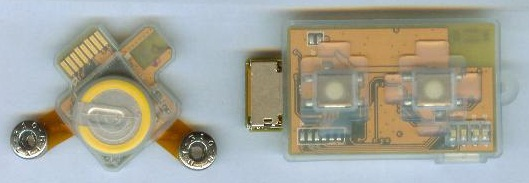
\includegraphics[scale=1]{truesense}
    \caption{Sensor y controlador TrueSense}
    \label{fig:truesense}
\end{figure}

\paragraph{
El sensor se conecta a electrodos que se ajustan con una banda elástica en cualquier zona del cuerpo.
}

\begin{figure}[ht]
    \centering
    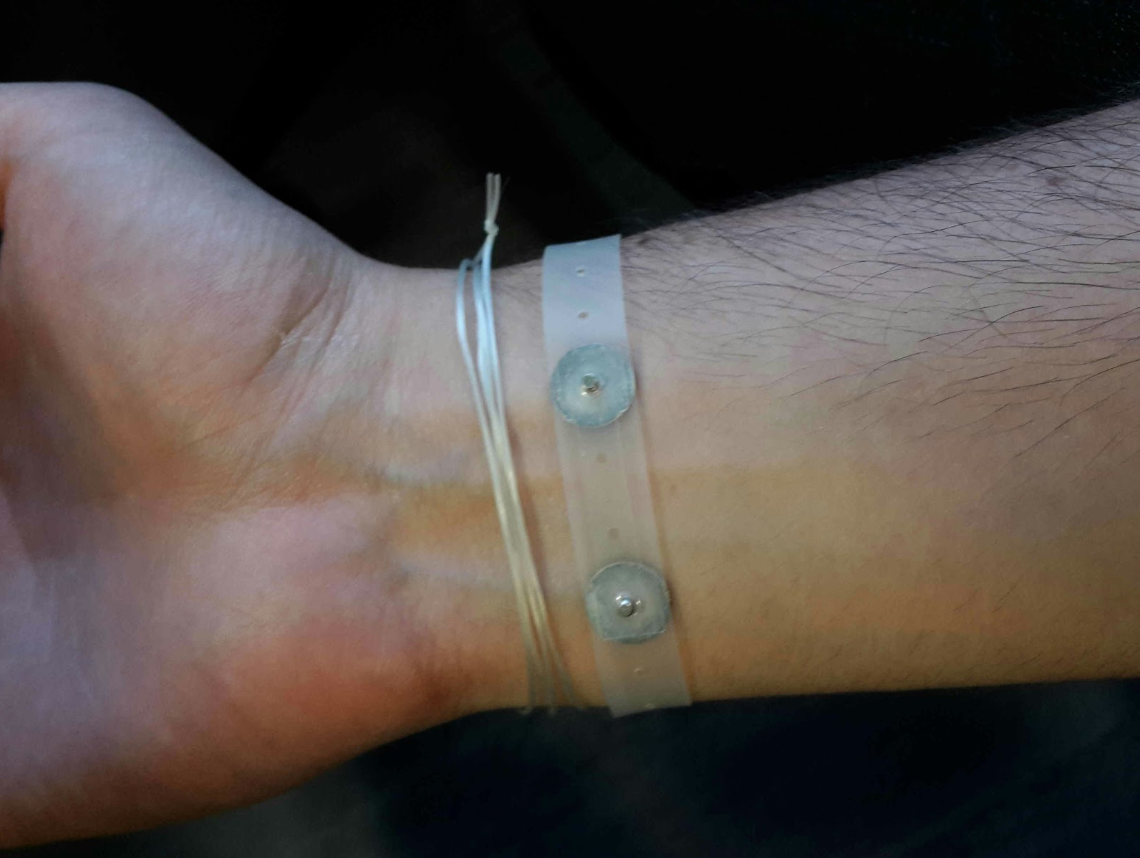
\includegraphics[height=2in]{electrodo_munieca.png}%
    \caption{Ubicación de los electrodos en la muñeca}
    \label{fig:electrodos1}
\end{figure}

\begin{figure}[ht]
    \centering
    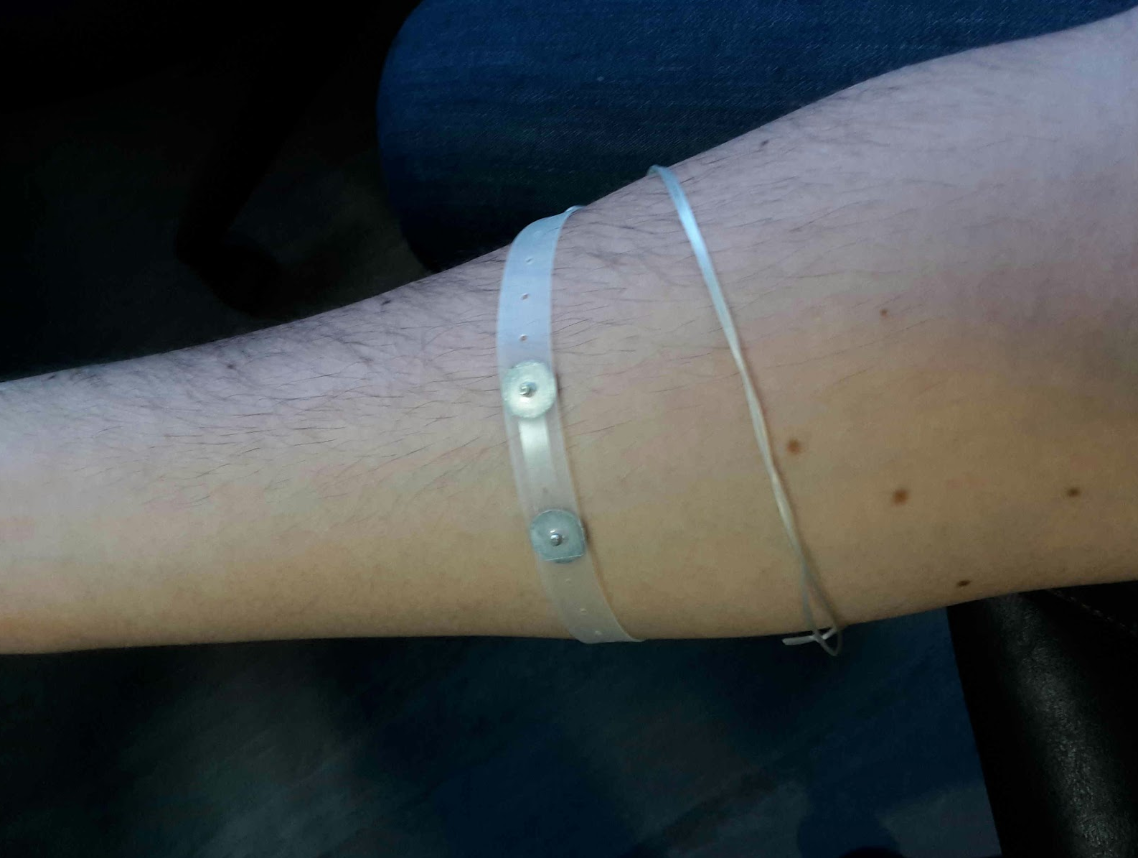
\includegraphics[height=2in]{electrodo_antebrazo.png}%
    \caption{Ubicación de los electrodos en el antebrazo}
    \label{fig:electrodos2}
\end{figure}

\paragraph{
Se tomaron muestras de distintos movimientos, entre ellos: cerrar y abrir la mano, flexionar muñecas y mover individualmente los dedos. La idea que se tenía era poder diferenciar dichos movimientos para que los usuarios pudieran crear contraseñas más complejas.
}
\paragraph{
Para probar la efectividad de la clasificación, en principio, se tomaron muestras que sólo contenían un único movimiento, para luego, en caso de una clasificación satisfactoria, probar si era posible detectar los movimientos en una señal compuesta por varios movimientos.
}
\paragraph{
Para clasificar los movimientos, se extrajeron las features para series de tiempo recomendadas en el paper \cite{angkoon2009}:
}

\begin{center}
\begin{tabular}{ c c }
 Integrated EMG & $IEMG = \sum_{n=1}^{N} \abs{X_n}$ \\
 Mean absolute value & $MAV = \frac{1}{N} \sum_{n=1}^{N} \abs{X_n}$ \\
 Simple Square Integral & $SSI = \sum_{n=1}^{N}\abs{X_n}^2$ \\
 Variance of EMG & $VAR = \frac{1}{N-1} \sum_{n=1}^{N} {X_n}^2$ \\
 Root mean square & $RMS = \sqrt{\frac{1}{N} \sum_{n=1}^{N} {X_n}^2}$ \\
 Waveform length & $WL = \sum_{n=1}^{N-1} \abs{X_{n + 1} - X_n}$
\end{tabular}
\end{center}

\paragraph{
En las [Figura \ref{fig:feature1}], [Figura \ref{fig:feature2}] y [Figura \ref{fig:feature3}] se pueden observar los resultados obtenidos de 20 muestras de los movimientos de cerrar dedos individualmente para distintas features.
}

\begin{center}
\begin{tabular}{ |c| }
\hline
    Referencias de nombres de los dedos en las figuras \\
\hline
    Finger 0: Dedo pulgar \\
    Finger 1: Dedo índice \\
    Finger 2: Dedo medio \\
    Finger 3: Dedo anular \\
    Finger 4: Dedo meñique \\
\hline
\end{tabular}
\end{center}

\begin{figure}[ht]
    \centering
    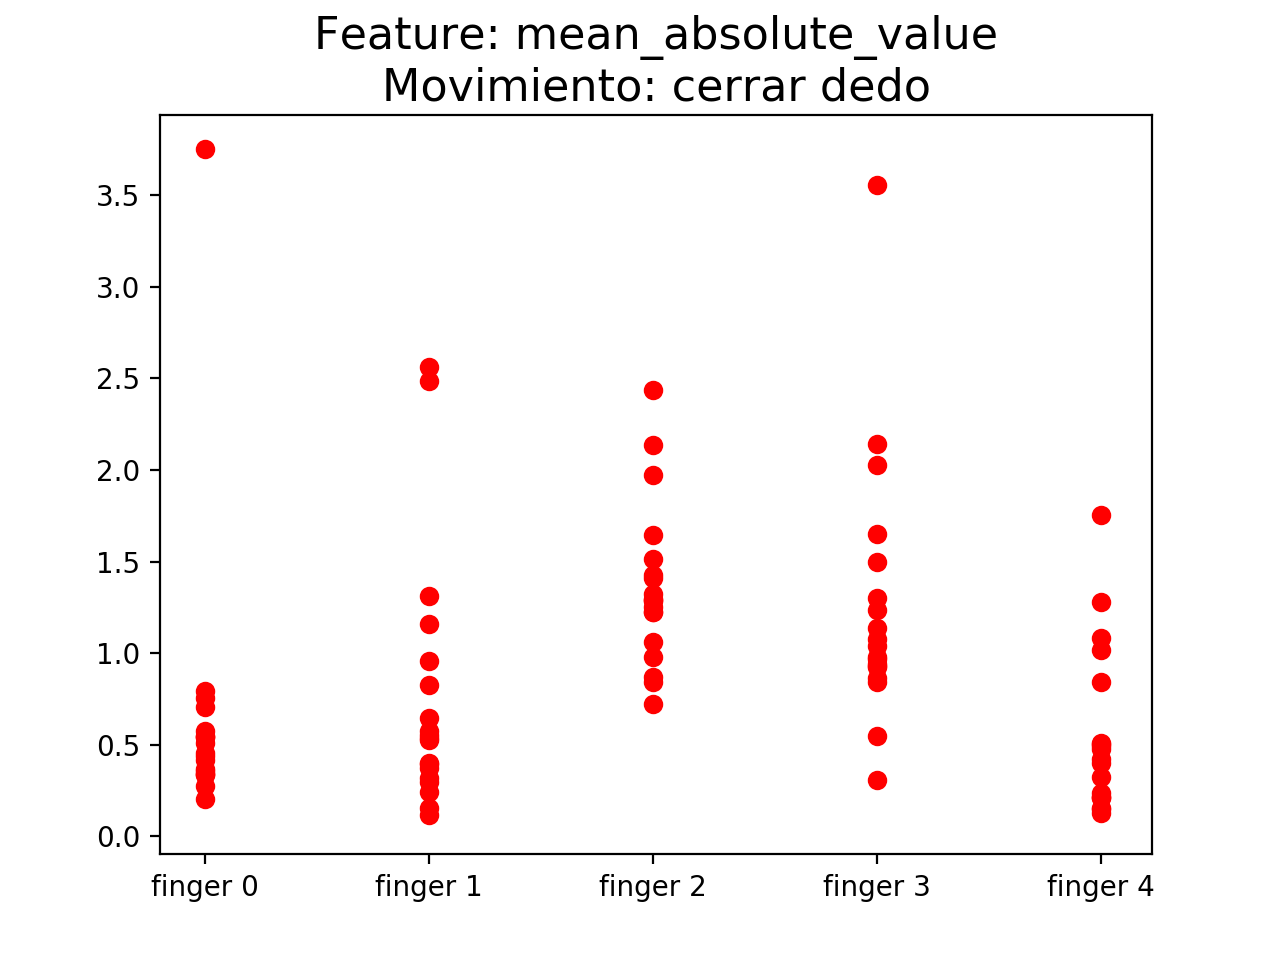
\includegraphics[width=\textwidth]{Figure_1.png}%
    \caption{Feature “mean absolute value” para los movimientos de cada dedo}
    \label{fig:feature1}
\end{figure}

\begin{figure}[ht]
    \centering
    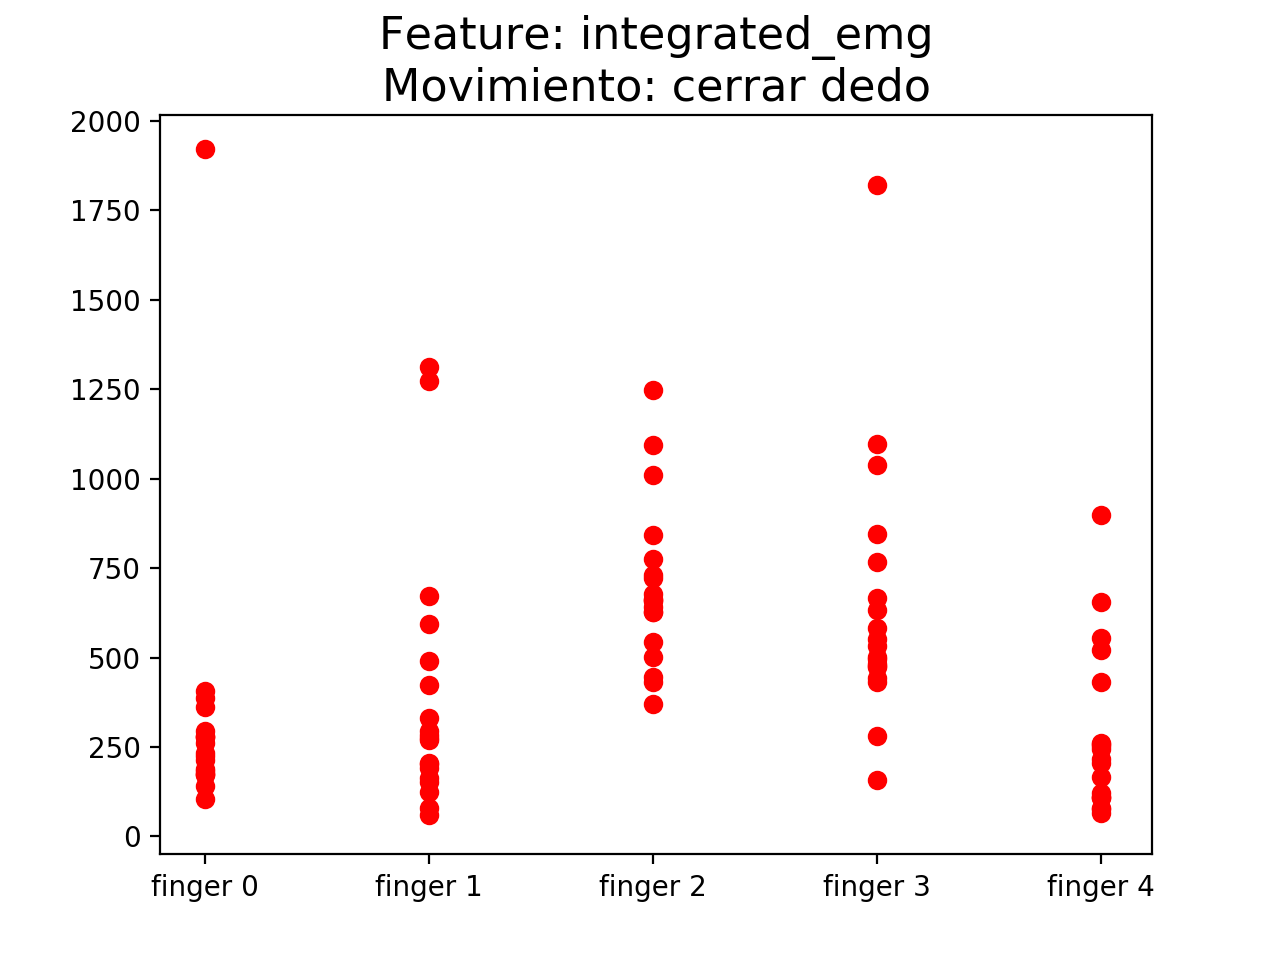
\includegraphics[width=\textwidth]{Figure_2.png}%
    \caption{Feature “integrated emg” para los movimientos de cada dedo}
    \label{fig:feature2}
\end{figure}

\begin{figure}[ht]
    \centering
    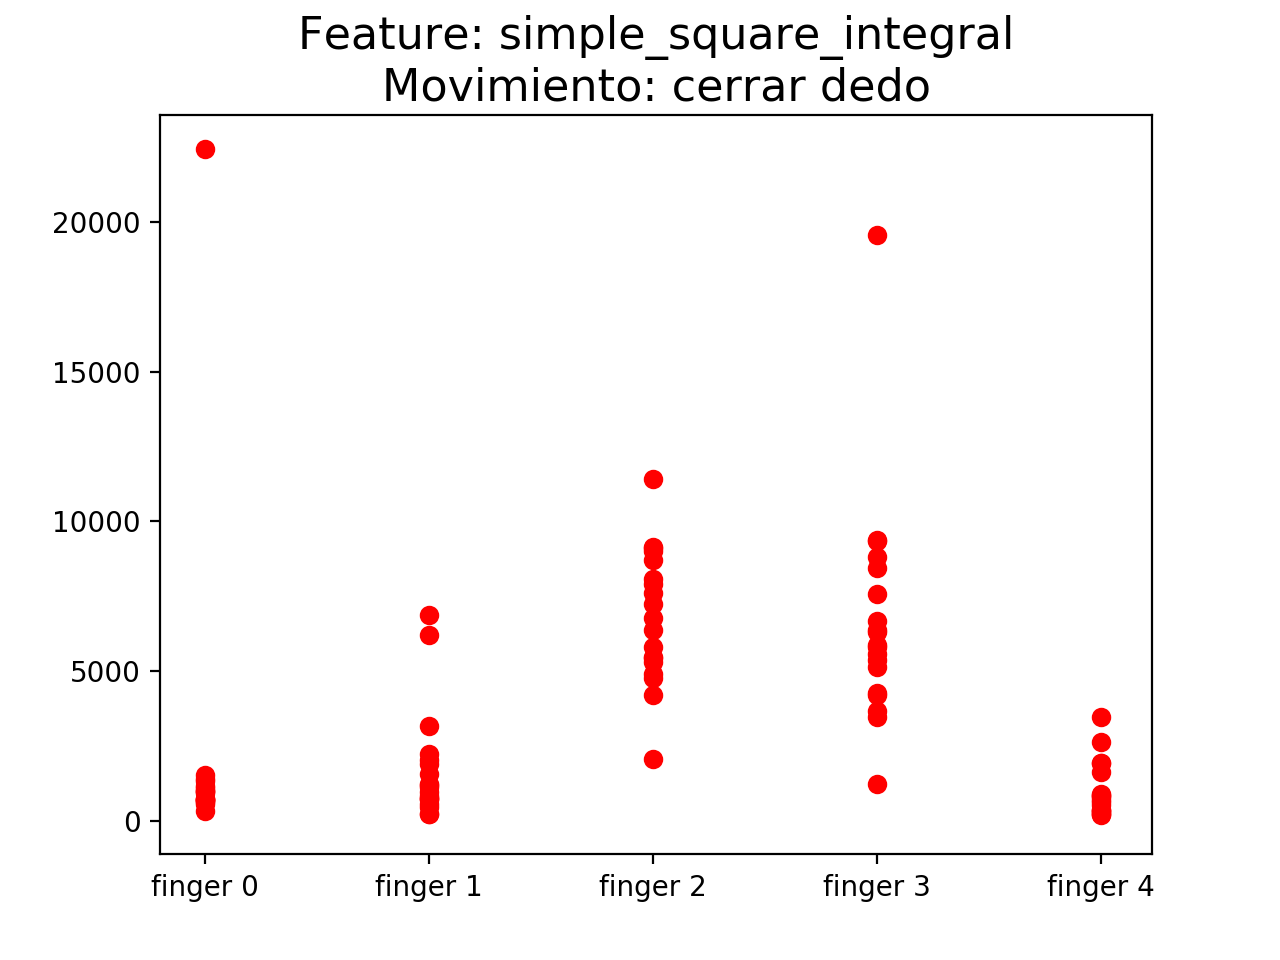
\includegraphics[width=\textwidth]{Figure_3.png}%
    \caption{Feature “simple square integral” para los movimientos de cada dedo}
    \label{fig:feature3}
\end{figure}

\paragraph{
Uno de los objetivos que debe tener un esquema de autenticación para conseguir la aceptación psicológica de los usuarios es que debe funcionar con poco entrenamiento por parte del mismo. Para esto, una buena opción podría ser utilizar un clasificador naive de Bayes. Tomamos como referencia el trabajo hecho en \cite{yousefi2015}, creando un clasificador para cada dedo utilizando porcentajes variables del total de muestras como set de pruebas (de 20\% a un 100\%) y el restante como set de entrenamiento. Esto no arrojó buenos resultados, y es por eso que decidimos utilizar las señales para la creación de contraseñas (mediante una transformación).
}

\subsection{Olimex EMG/EEG Shield}

\begin{figure}[ht]
    \centering
    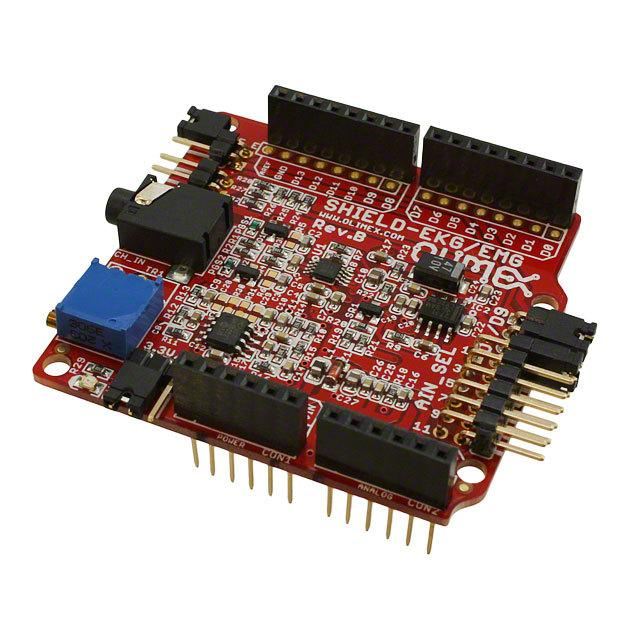
\includegraphics[width=2in]{SHIELD-EKG-EMG.jpg}%
    \caption{Fotografía de un Olimex EMG Shield}
    \label{fig:olimexshield}
\end{figure}

\paragraph{
El Olimex EMG/EEG Shield [Figura \ref{fig:olimexshield}] es una placa diseñada por la empresa Olimex que permite leer señales EMG o EEG desde un Arduino. Para hacer esto se deben conectar los electrodos deseados a la placa y la placa al Arduino. La placa se encarga de convertir la señal diferencial analógica (bioseñal) de los canales de entrada positivo y negativo, en un stream de datos como salida. Este stream puede ser leído por el Arduino mediante los pines analógicos. El Arduino se encarga de discretizar la señal y escribirla en el puerto serie.
}

\paragraph{
La colocación de los electrodos es bastante simple como se ve en la [Figura \ref{fig:colocacion-de-electrodos}], tienen una banda elástica de tela que permite una buena adherencia en los brazos. Es importante que el electrodo diferencial (rotulado con la letra ``D'' en este caso) este alejado de los otros dos electrodos, en nuestras pruebas lo colocamos en el brazo contrario a los demás. Los electrodos que miden la diferencia de potencial (rotulados con las letras ``R'' y ``L'') deben colocarse juntos en el mismo músculo. Aplicar alcohol sobre la piel en el lugar donde se sitúan los electrodos mejora la lectura de la señal.
}

\begin{figure}[ht]%
\centering
\subfigure[][]{%
\label{fig:coloc_elec_1}%
\includegraphics[height=2in, width=2in]{colocacion_electrodos_1.png}}%
\hspace{8pt}%
\subfigure[][]{%
\label{fig:coloc_elec_2}%
\includegraphics[height=2in, width=2in]{colocacion_electrodos_2.png}} \\
\subfigure[][]{%
\label{fig:coloc_elec_3}%
\includegraphics[height=2in, width=2in]{colocacion_electrodos_3.png}}%
\hspace{8pt}%
\subfigure[][]{%
\label{fig:coloc_elec_4}%
\includegraphics[height=2in, width=2in]{colocacion_electrodos_4.png}}%
\caption[]{
\subref{fig:coloc_elec_1} Electrodos EMG que se conectan a la Olimex Shield;
\subref{fig:coloc_elec_2} Los electrodos tienen una banda elástica que permite una buena adherencia al cuerpo;
\subref{fig:coloc_elec_3} Se coloca el; y,
\subref{fig:coloc_elec_4} Electrodos EMG.}%
\label{fig:colocacion-de-electrodos}%
\end{figure}

\subsection{Muse headband}
\begin{figure}[ht]
    \centering
    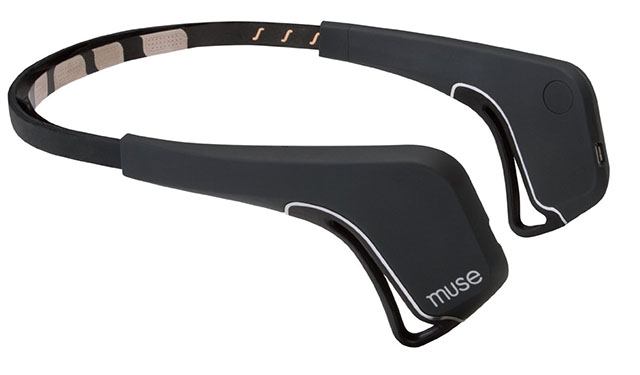
\includegraphics[width=2in]{museheadband.jpg}%
    \caption{Imagen de un Muse headband}
    \label{fig:muse}
\end{figure}
\paragraph{
Este es un dispositivo pensado para el monitoreo señales de EEG durante la meditación [Figura \ref{fig:muse}]. El dispositivo se conecta mediante Bluetooth LE (4.0) con un teléfono que tenga la aplicación de Muse, desde esta se pueden ver distintas métricas de las señales.}
\paragraph{
Del sitio web de Muse se encuentra disponible para descargar un SDK para iOS, Android y Windows 10 y un proyecto de Visual Studio 2015 de una aplicación para visualizar la señal.
}

\paragraph{
La identificación unívoca de una persona mediante señales de EEG como las del Muse es muy compleja, y se obtuvieron porcentajes de clasificación aún peores que los obtenidos con el TrueSense. La manipulación de forma volitiva de estas señales es muy complicada por lo que es casi imposible utilizarlas para generar una contraseña. El Muse cuenta con un acelerómetro interno que si puede ser utilizado para codificar una señal pero estos movimientos son más incómodos de realizar comparados con los posibles mediante los dispositivos de EMG. Estos valores pueden ser de mayor utilidad en una aplicación para personas con discapacidades motoras.
}

\subsection{Comparación}
\subsubsection{TrueSense}
\paragraph{
Durante las pruebas del dispositivo nos encontramos con que la batería del sensor tiene una duración de aproximadamente 20 minutos, además de tener que reiniciar la captura de señales por errores de calibración del dispositivo. Estos motivos hicieron que no se pudieran tomar muestras de forma consistente.
}
\subsubsection{Olimex EMG/EEG Shield}
\paragraph{
El Olimex Shield presenta una serie de ventajas ante True Sense como no necesitar baterías, lo que hace mucho menos tedioso realizar pruebas que se prolonguen en el tiempo. Debido a que se puede conectar cualquier electrodo, se pueden utilizar unos que se adhieran mejor a la piel y generen menos ruido. También la lectura por el puerto serie es mucho más simple y es posible definir una frecuencia de muestreo.
}
\subsubsection{Muse Headband}
\paragraph{
El Muse presentaba una serie de ventajas como ser fácil de colocar y una buena duración de la batería. Pero como desventajas tiene que, debido a que fue diseñado para ser utilizado desde un dispositivo móvil, la comunicación desde una computadora es dificultosa siendo Windows 10 el único sistema operativo soportado. Por ejemplo para poder obtener las señales desde la Raspberry PI que utilizamos en el prototipo era necesario portar todo el código del SDK.
}
\paragraph{
Las señales con participación activa del usuario que pueden obtenerse mediante el acelerómetro interno resultan más incomodas para el usuario que las generadas con el Olimex Shield.
}
\subsubsection{Conclusión}
\paragraph{
De los dispositivos disponibles decidimos quedarnos con el Olimex Shield ya que el mismo supera ampliamente al TrueSense en la facilidad de aplicación de los electrodos y no tiene los problemas de batería del anterior. El Muse presentaba una alternativa interesante por ser ya un producto de uso comercial, lo que se puede observar en su apariencia y facilidad de uso (no desarrollo). Al no poder obtener características que sirvan para identificar unívocamente a una persona se optó por generar una contraseña a partir de las señales. De los tres dispositivos probados, el que presentaba un mejor equilibrio entre comodidad para el usuario y facilidad de clasificación de la misma fue el Olimex Shield.
}

\section{Análisis de la señal EMG}
\paragraph{
En esta sección se describirá como fue el análisis de las señales obtenidas por el Olimex Shield EEG/EMG.
}
\paragraph{
El análisis de la señal consiste en dos partes, el preprocesamiento y la codificación. La señal cruda que proviene del dispositivo consiste en la diferencia de potencial entre los electrodos derecho e izquierdo. Con los electrodos colocados sobre un músculo en particular, los picos en la señal reflejan la activación del mismo.
}

\paragraph{
El en Olimex Shield, el rango de valores de la señal es de 0 a 5 volts mapeado a valores enteros de 0 a 1023 y la frecuencia de muestreo es de 256 Hz.
}

\begin{figure}[ht]
    \centering
    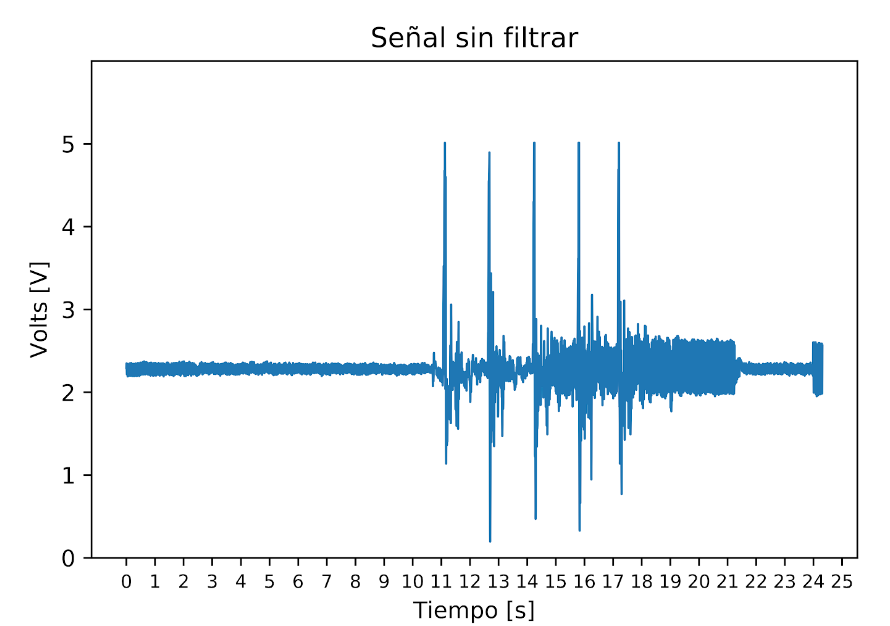
\includegraphics[width=\textwidth]{no-filter.png}%
    \caption{Ejemplo de una señal no filtrada obtenida}
    \label{fig:no-filter}
\end{figure}

\paragraph{
El objetivo es intentar encontrar picos en la señal, es decir, momentos en los que la persona haya realizado algún movimiento que produjo un cambio de potencial.
}
\paragraph{
La señal sera dividida en partes o \textit{ventanas} de longitud N configurables. Como el dispositivo tiene una frecuencia de muestreo de 256 Hz, una ventana de 256 valores representa la señal en un período de 1 segundo. El valor que se le da a N es importante ya que afecta directamente a la experiencia de usuario: un valor grande hará que la persona tenga un control más preciso pero que la duración del proceso sea más lento, mientras que un valor muy pequeño hará que el usuario pierda precisión y aumente la velocidad del proceso. Luego se aplicará el filtro de la ecuación (\ref{eq:filter}) a cada ventana, este filtro calcula el máximo de la señal \textit{s} en una ventana de dimensión \textit{n}  que mira hacia atrás a partir de la muestra \textit{i} de la señal
}

\begin{equation}\label{eq:filter}
f(s, i, n) = max(\big\{ s(x) : x = i - n, ..., i\big\})
\end{equation}



\paragraph{
El resultado visible de este filtro es que se logra una especie de señal "cuadrada", ya que nos quedamos con el máximo valor de cada una de las ventanas [Figura \ref{fig:filtered}].
}

\begin{figure}[ht]
    \centering
    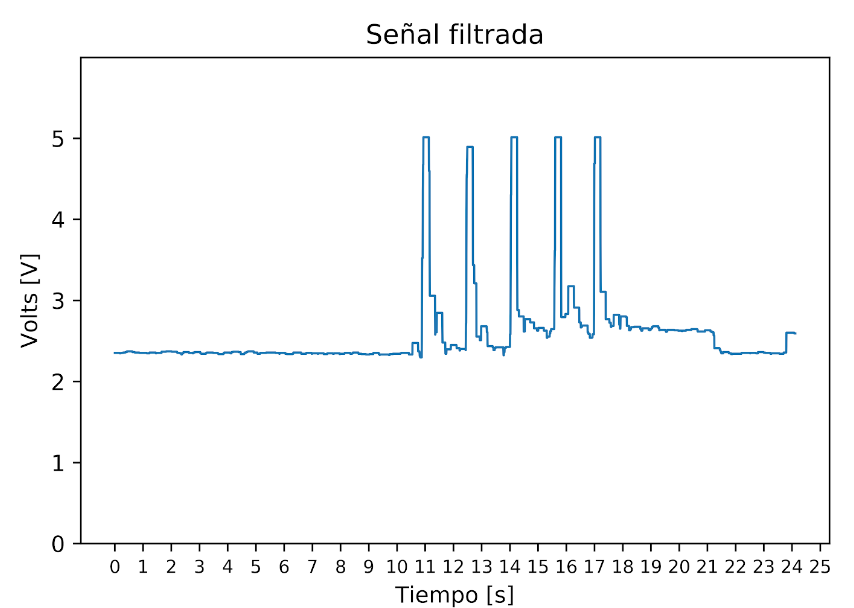
\includegraphics[width=\textwidth]{filtered.png}%
    \caption{Resultado de filtrar la señal de la figura \ref{fig:no-filter}. Se puede observar menos ruido y se aprecian mejor los picos de activación. La ventana utilizada fue de 50 muestras, que con una frecuencia de muestreo de 256 Hz da una duración de aproximadamente 0.2 segundos.}
    \label{fig:filtered}
\end{figure}


\begin{figure}[ht]
    \centering
    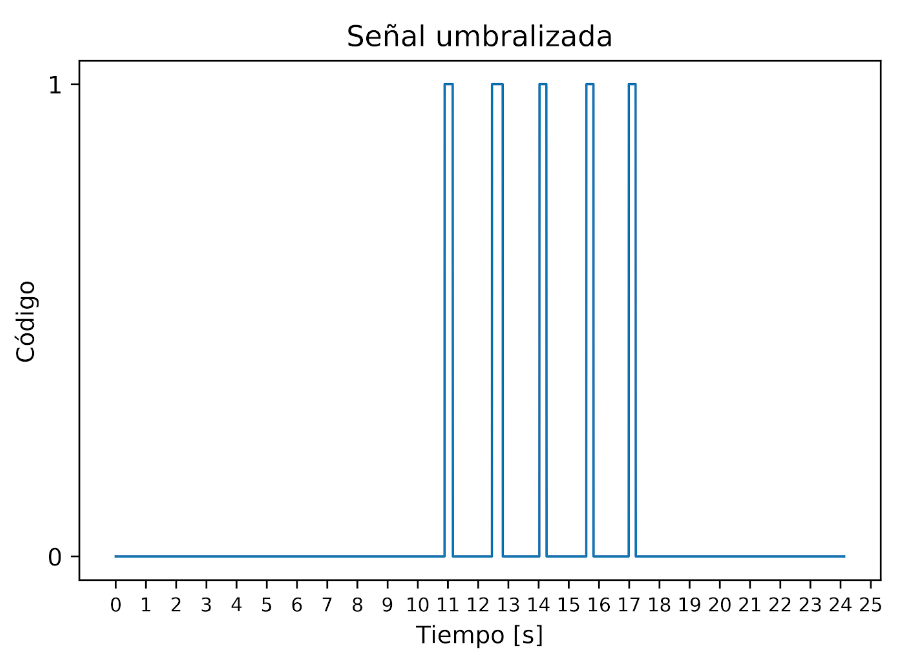
\includegraphics[width=\textwidth]{umbralized.png}%
    \caption{Resultado de umbralizar la señal de la figura. El umbral elegido fue de 650 lo que serian unos 3.185 volts.
    \ref{fig:filtered}}
    \label{fig:umbralized}
\end{figure}

\paragraph{
La segunda etapa de análisis consiste en transformar la señal a un código binario, siendo 1 un pico de activación y 0 el reposo. Para esto se debe elegir un valor de umbral, el cual hace que todos los valores por debajo del mismo se transformen en 0 y todos los valores superiores se transformen en 1, de esta manera detectar un cambio se vuelve muy simple y podemos generar el código binario [Figura \ref{fig:umbralized}].
}
\subsection{Comparación de las señales}
\paragraph{
Una vez transformadas las señales en cadenas de bits, lo que nos queda es conseguir una manera de diferenciar dos señales.
}
\paragraph{
Dado que la señal ahora es binaria, se puede utilizar cualquier método existente en las telecomunicaciones y se eligió utilizar la distancia de Hamming. Esta se define como el número de bits que tienen que cambiarse para transformar una palabra de código válida en otra palabra de código válida.
}
\paragraph{
Para calcular dicha distancia hay que sumar la cantidad de bits que difieren de una palabra respecto a la otra. Definimos la diferencia entre dos señales en la ecuación [\ref{eq:hamming}], siendo $B$ la cantidad de bits diferentes y $L_{1}$ y $L_{2}$ las longitudes de las señales.
}

\begin{equation}\label{eq:hamming}
D(L_1, L_2, B) =
\Bigg\{
  \begin{tabular}{ c c }
  $ 0 $ & si $L_1 \neq L_2$ \\
  $1 - \frac{B}{L_1}$ & si $L_1 = L_2$
  \end{tabular}
\end{equation}

\section{BAD API}
\paragraph{
Agregar un multifactor que utilice bioseñales a un sitio existente no es algo simple de hacer, por eso es una buena idea utilizar un servicio externo que permita hacerlo de la forma más simple posible.
}
\paragraph{
Luego de la investigación realizada, se decidió implementar un esquema testigo completo de autenticación por segundo factor basado en señales de EMG.  La solución incluye un servicio SaaS que provea una forma de agregar una autenticación reutilizable desde cualquier tipo de aplicación externa. A este servicio lo llamamos BAD API (Biosignal Authentication Device) y la idea es que sea un servicio Cloud Platform As A Service que puedan utilizar clientes en sus aplicaciones. Los clientes de este servicio no son los usuarios finales de un sistema, sino que son, en principio, los proveedores de servicios web (por ejemplo el home banking de un banco) que deseen agregar este tipo de segundo factor para sus usuarios.
}
\paragraph{
El servicio BAD API proveerá a los clientes de los dispositivos que leen las señales EMG y cuenta con un servidor en la nube que los mismos pueden utilizar para conectarse. Para esta conexión es necesario un access key que se proveerá a los clientes junto con los dispositivos.
}
\paragraph{
En los siguientes apartados se explicarán todos los detalles y fundamentos técnicos del servicio.
}

\subsection{Arquitectura}
\paragraph{
El servicio cloud utilizado para desplegar la BAD API y para comunicar de forma segura los dispositivos fue Google Cloud Platform, mas precisamente sus servicios IoT Core \cite{GoogleIotCore}, App engine \cite{GoogleAppEngine} y Cloud SQL \cite{GoogleCloudSQL}.
}
\paragraph{
IoT Core es un servicio que permite administrar dispositivos IoT y que los mismos se comuniquen de forma segura. Cada dispositivo debe tener un par de claves pública y privada y debe estar registrado en la consola web que provee Google con su clave pública. Los dispositivos que no utilizan una clave registrada tienen el acceso denegado.
}

\begin{figure}[ht]
    \centering
    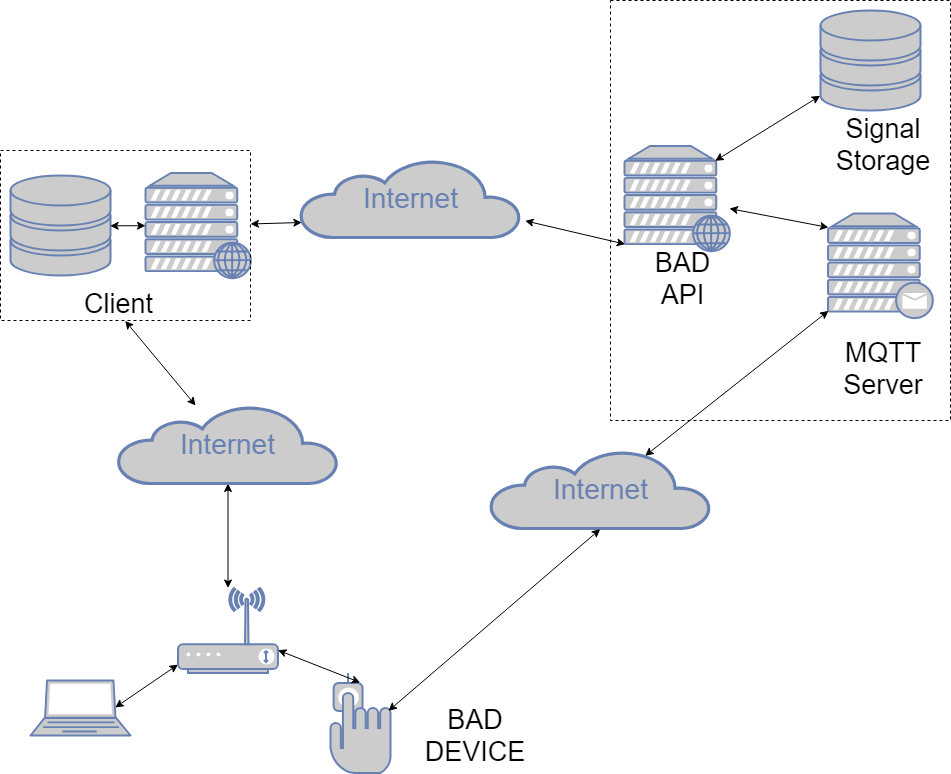
\includegraphics[width=\textwidth]{diagrama_general.png}%
    \caption{Diagrama general}
    \label{fig:generaldiagram}
\end{figure}

\subsection{Comunicación}
\paragraph{
Los dispositivos envían las señales y el estado de los mismos utilizando el protocolo MQTT y enviando la información de forma encriptada utilizando TLS. Este protocolo permite crear canales de comunicación en los que los agentes pueden publicar y otros pueden suscribirse. En este caso los dispositivos publican y la BAD API se suscribe para recibir la información y guardarla en la base de datos.
}
\paragraph{
El servicio IoT Core de Google permite a los suscriptores de los canales poder obtener información sobre los autores de los mensajes de manera automática, por lo tanto, no es necesario enviar esa información en los mensajes.
}

\subsection{MQTT}
\paragraph{
El protocolo de comunicación utilizado para la comunicación entre los dispositivos y el servicio cloud es el MQTT (Message Queuing Telemetry Transport). Es un protocolo del tipo \textit{publish-subscriber} que funciona sobre TCP/IP.
}
\paragraph{
Para comunicarse es necesario que exista al menos una cola de mensajes o ``canal'' a la cual un agente se suscribe y otro publica. El protocolo en si mismo es simple y agrega muy poco \textit{overhead} a los mensajes, por lo tanto el tamaño del mensaje es casi en su totalidad la información que se desea enviar. Esto último es principalmente útil en nuestro caso dado que sera utilizado por dispositivos IoT que tienen poco poder de procesamiento y probablemente conexiones a internet con poco ancho de banda.
}
\paragraph{
El servicio IoT Core de Google permite a los suscriptores de los canales poder obtener información sobre los autores de los mensajes de manera automática, por lo tanto, no es necesario enviar esa información en los mensajes.
}

\subsubsection{Canal “Status”}
\paragraph{
Uno de los aspectos que le interesan a la BAD API es la IP que tienen los dispositivos, ya que los usuarios se comunicarán con los mismos mediante la interfaz web expuesta en dicha IP. Para esto, existe un canal del protocolo MQTT exclusivo llamado “status” y tiene como objetivo enviar información del estado del dispositivo. En esta primera versión únicamente se utiliza para enviar la dirección IP de los dispositivos. En implementaciones futuras se podría agregar más información útil para detección de errores. El mensaje actual es el siguiente:
}
\begin{minted}[frame=single,
               framesep=3mm,
               xleftmargin=21pt,
               tabsize=4]{js}
{
    "IP": "192.169.0.11"
}
\end{minted}

\subsubsection{Canal “Signal”}
\paragraph{
Este canal se utiliza para enviar la señal a la BAD API. El mensaje actual es el siguiente:
}
\begin{minted}[frame=single,
               framesep=3mm,
               xleftmargin=21pt,
               tabsize=4]{js}
{
    "uuid": "9583cd17-9f85-4eac-8099-17fb3ab203b7",
    "Signal": [0, 1, 0, 1, 1, 0]
}
\end{minted}

\subsection{Comunicación entre los usuarios, clientes y la BAD API}
\paragraph{
El protocolo de comunicación principal elegido fue HTTPS, lo que facilita la integración por parte de los clientes. Actualmente la conexión entre el cliente y la BAD API se utiliza con HTTPS con el certificado de Google mientras que la comunicación entre el usuario y los dispositivos se realiza mediante HTTPS con certificados cruzados autofirmados.
}

\begin{figure}[ht]
    \centering
    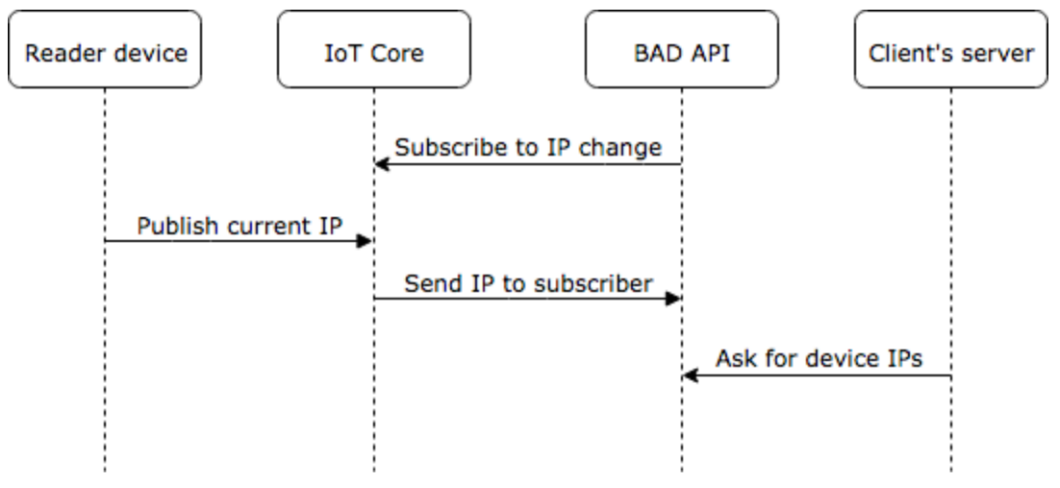
\includegraphics[width=\textwidth]{ipexchange.png}%
    \caption{Flujo de comunicación de la IP del dispositivo}
    \label{fig:ipexchange}
\end{figure}

\begin{figure}[ht]
    \centering
    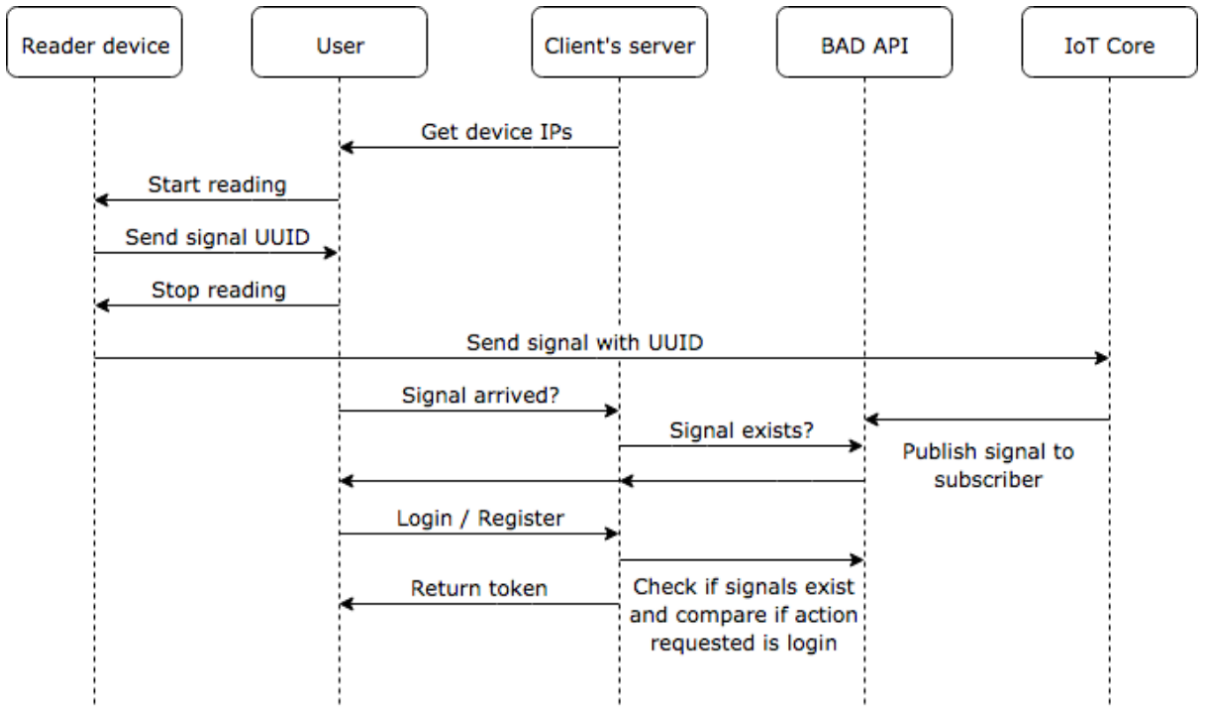
\includegraphics[width=\textwidth]{authschema.png}%
    \caption{Esquema de autenticación utilizando el servicio de BAD API}
    \label{fig:authschema}
\end{figure}

\paragraph{
En principio, la aplicación cliente le despliega al usuario, las opciones de dispositivos que tiene disponibles para él [Figura \ref{fig:ipexchange}]. Dado que el cliente tiene toda la información de sus dispositivos, este puede mostrarle la información a sus usuarios a criterio, como puede ser sólo los dispositivos cercanos.
}
\paragraph{
El usuario elige uno de los dispositivos disponibles y puede pedirle que comience a leer la señal, obteniendo un UUID que la representará en la BAD API.
}
\paragraph{
Cuando el dispositivo recibe la señal informando una interrupción en la lectura, éste pública la misma en el canal MQTT provisto por el servicio cloud, el cual será recibido por la BAD API.
}
\paragraph{
Una vez que la señal fue recibida por la BAD API, el usuario le envía al servicio cliente un request para registrarse o loguearse [Figura \ref{fig:authschema}].
}
\paragraph{
Es aqui el unico punto en donde difieren ambos flujos:
}
\begin{itemize}
    \item Para el caso del registro, el servicio cliente solo verifica que la señal exista en la BAD API y no haya sido utilizada por algún otro usuario, en caso afirmativo el cliente guarda la información del usuario y el UUID de la señal con la que se registro.
    \item Para el caso del login, el cliente envía el UUID de la señal recién obtenida y el UUID de la señal de registro que tiene en su sistema a la BAD API para que las compare. Este último le envía un porcentaje de similitud entre ambas señales. El servicio cliente decide que hacer dado el porcentaje recibido (podrá denegar el login si es muy bajo o mostrar parte del contenido).
\end{itemize}


\subsection{BAD-DEVICE-I: Prototipo del dispositivo}
\paragraph{
Para el primer prototipo se decidió utilizar dispositivos electrónicos de uso general (esto permite realizar modificaciones del prototipo de forma rápida y económica). Se utilizó una Raspberry PI a la cual se conectó un Arduino Chipkit Uno32 con un Shield EMG de Olimex, el cual se conecta a un sensor EMG de 3 electrodos: derecho (R) izquierdo (L) y diferencial (D). La señal obtenida consiste en la diferencia de potencial entre los electrodos derecho e izquierdo tomando como tierra el diferencial.
}
\paragraph{
Para mejorar la calidad de la señal es recomendable aplicar alcohol sobre la piel en el lugar donde se sitúan los electrodos ya que esto reduce la impedancia de la piel
\cite{sanei2007}.}

\begin{figure}[ht]%
\centering
\subfigure[][]{%
\label{fig:ex3-a}%
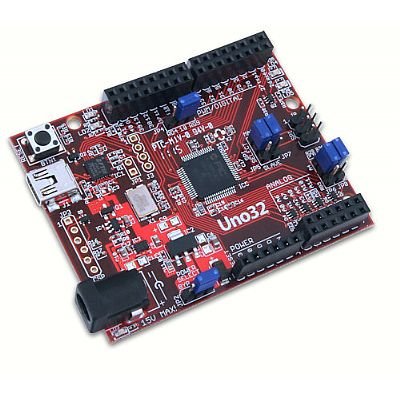
\includegraphics[height=2in, width=2in]{arduino.jpg}}%
\hspace{8pt}%
\subfigure[][]{%
\label{fig:ex3-b}%
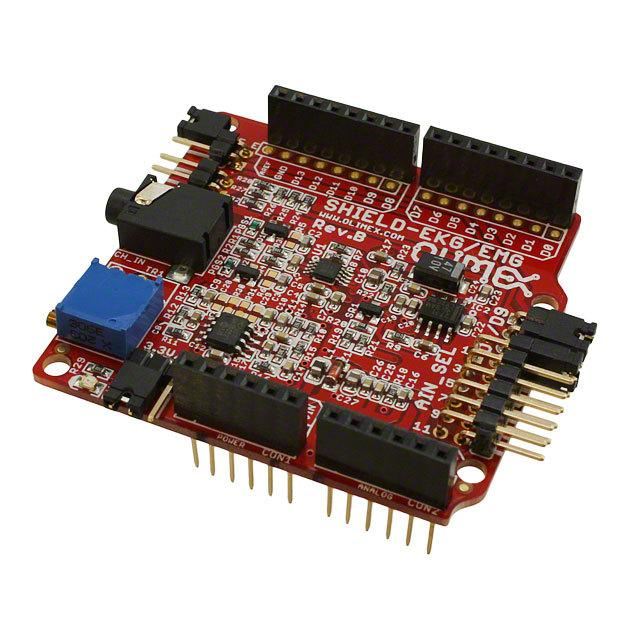
\includegraphics[height=2in, width=2in]{SHIELD-EKG-EMG.jpg}} \\
\subfigure[][]{%
\label{fig:ex3-c}%
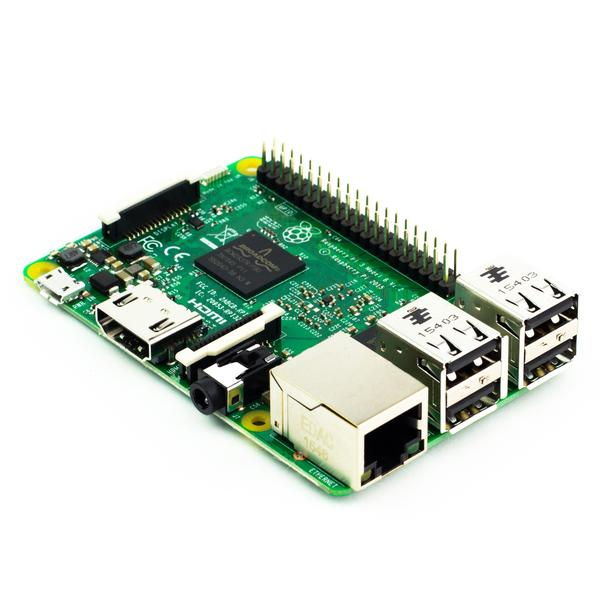
\includegraphics[height=2in, width=2in]{RPI3.JPG}}%
\hspace{8pt}%
\subfigure[][]{%
\label{fig:ex3-d}%
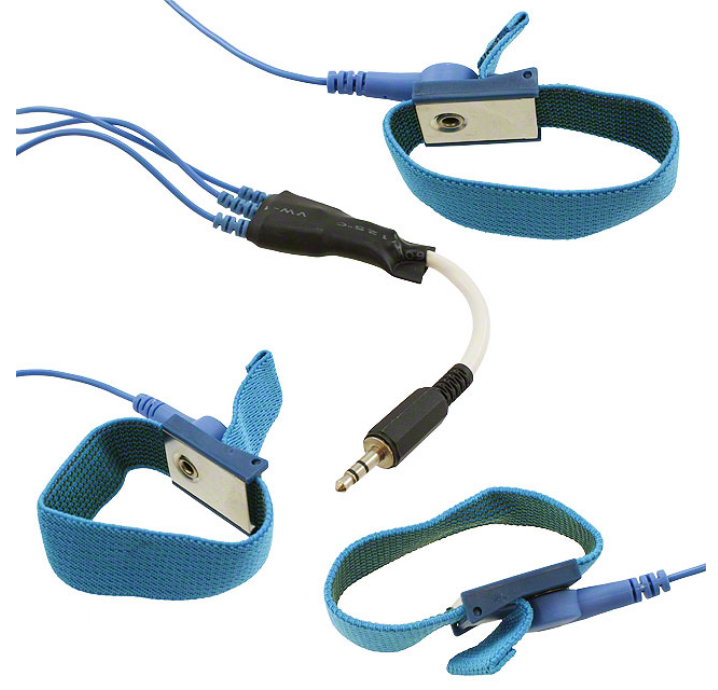
\includegraphics[height=2in, width=2in]{electrodos.png}}%
\caption[]{
\subref{fig:ex3-a} Arduino Chipkit Uno32;
\subref{fig:ex3-b} Olimex EMG/EEG Shield;
\subref{fig:ex3-c} Raspberry Pi 3; y,
\subref{fig:ex3-d} Electrodos EMG.}%
\label{fig:ex3}%
\end{figure}

\paragraph{
La Raspberry tiene instalado un servidor web que expone una API JSON que permite a los clientes comunicarse fácilmente mientras que sus usuarios se encuentren en la misma red. En caso de exponer la Raspberry con una IP publica, el dispositivo podría ser accedido desde cualquier lugar.
}
\paragraph{
Los parametros de la umbralización de la señal son configurables por el usuario. Esto permite que la lectura de la señal se adapte a cada usuario, lo cual es muy importante debido a la señal es variable de manera intrapersonal.
}
\paragraph{
Además, la Raspberry posee el software y la clave privada necesarios para comunicarse con la BAD API a través de internet de forma segura. Dicha clave estará preconfigurada antes de entregar el dispositivo al cliente y la clave pública asociada estará registrada en el servicio web.
}

\subsection{Integración por parte de los clientes}
\paragraph{
Los clientes del servicio BAD deberán primero obtener un access key para comunicarse con la API. Estas keys se proveerán de forma directa luego de la contratación del servicio.
}
\paragraph{
Una vez contratado el servicio, los clientes deben desarrollar una integración con las interfaces HTTPS del dispositivo y de la API.
}
\paragraph{
La documentación de ambas interfaces se detalla en el siguiente apartado. Tanto la documentación como una aplicación de prueba se mostrarán de forma pública para que los clientes puedan realizar la integración sin problemas.
}

\subsection{Interfaz BAD API}
\paragraph{
Esta API expone una interfaz de comunicación mediante el protocolo HTTPS y el formato de los mensajes intercambiados es JSON. El envío del access key se realiza mediante el header “Authorization” de HTTPS.
}
\subsubsection{GET /api/v1/signals/:uuid}
\paragraph{
Este endpoint sirve para verificar la existencia de una señal en la base de datos.
}

\paragraph{
Parámetros de entrada:}
El único parámetro necesario es el uuid de la señal y se provee a través de la URL.
\paragraph{
Salida:}
El cuerpo de la salida es vacío, la información está en el código HTTPS de la respuesta.

\paragraph{
Códigos de respuesta posibles:
}
\begin{itemize}
    \item 204: la señal se encuentra en la base de datos.
    \item 404: la señal no se encuentra en la base de datos o el dispositivo que la tomó no le pertenece al cliente que realiza el pedido.
    \item 401: No se envió el access token o no le pertenece a ningún cliente.
\end{itemize}

\subsubsection{POST /api/v1/signals/compare}
\paragraph{
Este endpoint sirve para comparar dos señales pertenecientes a cualquier dispositivo de un cliente.
}

\paragraph{
Parámetros de entrada:}
Este endpoint requiere los uuid de las señales en el body de la request HTTPS:

\begin{minted}[frame=single,
               framesep=3mm,
               xleftmargin=21pt,
               tabsize=4]{js}
{
    "signal_1_uuid": "9583cd17-9f85-4eac-8099-17fb3ab203b7",
    "signal_2_uuid": "7c4bdfdf-e6f0-463d-aec5-ad3db7d815da"
}

\end{minted}

\paragraph{
Salida:}
Se devuelve un valor entre 0 y 1 que representa la similitud de las señales.

\begin{minted}[frame=single,
               framesep=3mm,
               xleftmargin=21pt,
               tabsize=4]{js}
{
    "percentage": 0.834
}
\end{minted}

\paragraph{
Códigos de respuesta posibles:
}
\begin{itemize}
    \item 200: el pedido fue satisfactorio.
    \item 404: alguna de las señales no se encuentra en la base de datos o el dispositivo que las tomó no le pertenece al cliente que realiza el pedido.
    \item 401: No se envió el access token o no le pertenece a ningún cliente.
\end{itemize}

\subsubsection{GET /api/v1/devices}
\paragraph{
Este endpoint le permite conocer a los clientes la información de sus dispositivos.
}
\paragraph{
Salida:
}

\begin{minted}[frame=single,
               framesep=3mm,
               xleftmargin=21pt,
               tabsize=4]{js}
[
    {
        "id": "mac-2",
        "ip_address": "192.168.0.179"
    },
    {
        "id": "rpi-1",
        "ip_address": "192.168.0.11"
    }
]

\end{minted}

\paragraph{
Códigos de respuesta posibles:
}
\begin{itemize}
    \item 200: el pedido fue satisfactorio.
    \item 401: No se envió el access token o no le pertenece a ningún cliente.
\end{itemize}

\subsection{Interfaz BAD-DEVICE-I}
\paragraph{
La interfaz expuesta en el prototipo también utiliza el protocolo HTTPS y JSON como formato de los mensajes.
}
\subsubsection{POST /api/v1/start}
\paragraph{
Este endpoint le indica al dispositivo que debe comenzar a leer una señal y devuelve el UUID que identificará a la misma.
}
\paragraph{
Salida:}

\begin{minted}[frame=single,
               framesep=3mm,
               xleftmargin=21pt,
               tabsize=4]{js}
{
    "signalUUID": "9583cd17-9f85-4eac-8099-17fb3ab203b7"
}
\end{minted}

\paragraph{
Códigos de respuesta posibles:
}
\begin{itemize}
    \item 201: el pedido fue satisfactorio y se crea el UUID de la señal.
\end{itemize}

\subsubsection{POST /api/v1/stop}
\paragraph{
Este endpoint le indica al dispositivo que debe parar de leer la señal y enviará la señal a través del protocolo MQTT a la BAD API.
}
\paragraph{
Salida:
}

\begin{minted}[frame=single,
               framesep=3mm,
               xleftmargin=21pt,
               tabsize=4]{js}
{
    "signalUUID": "9583cd17-9f85-4eac-8099-17fb3ab203b7"
}
\end{minted}

\paragraph{
Códigos de respuesta posibles:
}
\begin{itemize}
    \item 200: el pedido fue satisfactorio y se envió la señal a la BAD API.
\end{itemize}

\subsubsection{POST /api/v1/cancel}
\paragraph{
Este endpoint cancela la recolección de la señal actual sin enviar el resultado previo a la BAD API.
}
\paragraph{
Códigos de respuesta posibles:
}
\begin{itemize}
    \item 200: el pedido fue satisfactorio y se cancela la recolección de la señal.
\end{itemize}
\subsubsection{GET /api/v1/read}
\paragraph{
Este endpoint permite a la aplicación cliente ver los valores que están siendo leídos por el dispositivo. No es necesario utilizar este endpoint para el correcto funcionamiento del sistema, pero sirve para dar un feedback a los usuarios.
}
\paragraph{
\textbf{Salida}:
}
Se devuelve tanto los valores de la señal cruda como los valores de la señal codificada. El formato de ambas señales es de un array que contiene las coordenadas X e Y de la señal.


\begin{minted}[frame=single,
               framesep=3mm,
               xleftmargin=21pt,
               tabsize=4]{js}
{
    "signal": [[0, 123], [1, 657], [2, 456]],
    "Interpreted_signal": [[0, 0]]
}

\end{minted}
\paragraph{
Códigos de respuesta posibles
}
\begin{itemize}
    \item 200: el pedido fue satisfactorio.
\end{itemize}

\section{Threat model}
\paragraph{
En esta sección se describirán las posibles amenazas y los aspectos de seguridad relevantes en el sistema, así también como fueron mitigados algunas de las amenazas y cómo se pueden mitigar las demás.
}
\paragraph{
Hay cuatro canales de comunicación que manejan y/o almacenan información sensible [Figura \ref{fig:generaldiagram}].
}

\subsection{Comunicación entre el dispositivo y la computadora del usuario}
\paragraph{
Como hemos descripto anteriormente, el usuario se comunica con el dispositivo para avisarle que debe comenzar, parar o cancelar la lectura de la señal y este le responde con el ID de la señal. Además se transmite la señal para que el usuario pueda recibir feedback del proceso.
}
\paragraph{
Para que esta comunicación sea segura, se debe utilizar el protocolo HTTPS, por ende el dispositivo debe contar con un certificado X.509 firmado por una autoridad certificante que la computadora del usuario confíe. Como la comunicación hacia la BAD API también debería utilizar TLS, se pueden generar certificados firmados por el certificado autorizado de la BAD API. Este certificado no esta disponible en la primera versión del prototipo.
}
\paragraph{
Si bien la comunicación se puede realizar de forma segura, queda un problema más: que un atacante puede observar la señal que se muestra como forma de feedback y luego intentar reproducirla. La única opción manejable por el servicio BAD API, es que no se envíe la señal a modo de feedback sino que el dispositivo de una señal (luces o similar) al usuario indicándole si está leyendo o no. Por lo tanto los clientes deben tomar los recaudos necesarios para que esto no suceda. Sería posible mostrarle al usuario una especie de tutorial (como el que tiene la aplicación de prueba) que permita al usuario personalizar la lectura, pero al momento del registro de la señal se oculte en la pantalla el feedback.
}
\subsection{Entre el servidor del cliente y la BAD API}
\paragraph{
La comunicación entre ambos se realiza mediante el protocolo HTTPS, donde el cliente debe enviar un \textit{access key} generado de forma segura por la BAD API. Este último aspecto le permite a la BAD API denegar el acceso a cualquier otro servicio que quiera impersonificar al cliente, sin embargo, el guardado de esta clave de forma segura queda en manos del cliente. Se recomienda que se guarde de forma encriptada, o en variables de entorno del servidor teniendo un estricto control de quienes pueden acceder a las mismas.
}
\subsection{Entre el dispositivo y la BAD API}
\paragraph{
Si bien se utiliza el protocolo MQTT, que no tiene una transmisión segura, el servicio de Google Cloud le agrega una capa de seguridad al mismo. Los mensajes viajan encriptados al servidor utilizando TLS, previo a una autenticación realizada con criptografía asimétrica (el dispositivo genera un \textit{JWT} firmado con la clave privada, el cual es verificado por Google con la clave pública previamente guardada [Figura \ref{fig:tokencreation}]).
}

\begin{figure}[ht]
    \centering
    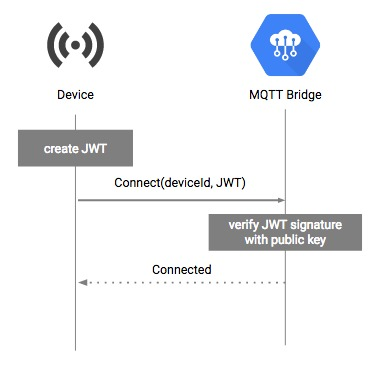
\includegraphics[width=3in]{token-creation.jpeg}%
    \caption{Autenticación de los dispositivos frente a Google Cloud}
    \label{fig:tokencreation}
\end{figure}

\paragraph{
El registro de la clave pública del dispositivo en los servicios de Google se realizan a nombre de la BAD API y sólo pueden hacerse de forma autenticada [Figura \ref{fig:keypairgeneration}]. Tanto el registro como el guardado de la clave pública en el dispositivos son realizados por desarrolladores de la BAD API y no se guarda ningún tipo de copia de la clave privada. La generación del par de claves se realiza con las recomendaciones de seguridad de Google \cite{GoogleIotSecurity}.
}

\begin{figure}[ht]
    \centering
    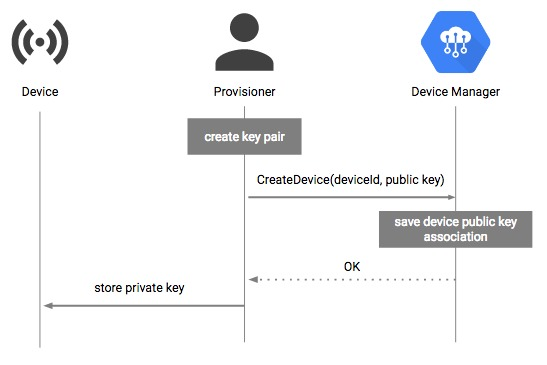
\includegraphics[width=3in]{key-generation.jpeg}%
    \caption{Distribución de claves}
    \label{fig:keypairgeneration}
\end{figure}

\paragraph{
Con estos recaudos, sin tener acceso a la clave privada, no es posible que un atacante envíe una señal artificial o altere una señal en tránsito.
}

\subsection{Entre la computadora del usuario y el servidor del cliente.}
\paragraph{
Esta conexión esta fuera del alcance de la BAD API y debería realizarse al menos utilizando HTTPS. Aquí también toma importancia el hecho de poder eliminar o expirar señales para evitar ataques de replay.
}
\subsection{Guardado del ID de la señal por parte del cliente}
\paragraph{
Los IDs de las señales son utilizados para enviarlos a la BAD API y que ésta las compare, por este motivo, el cliente debe conservar el valor del mismo sin alterarlo. Normalmente las contraseñas no se almacenan en texto plano ni encriptadas si no se necesita su valor, simplemente se guarda su hash. En este caso, debido a que se necesita el valor para enviarlo, se recomienda que se guarde el ID de forma encriptada.
}
\paragraph{
En este primer prototipo de la BAD API, las señales no tienen ningún tipo de expiración o forma de invalidar las mismas, por lo tanto, es recomendable que los clientes guarden una lista de los IDs que se usaron para logins en el pasado para evitar posibles replay attacks. En un futuro también sería posible agregar a la BAD API una manera de eliminar señales o de agregarle expiración a las mismas para evitar agregarle una carga extra a los clientes.
}
\subsection{Guardado de las claves y la señal en el dispositivo}
\subsubsection{Normas FIPS}
\paragraph{
FIPS es un estándar de seguridad para módulos criptográficos que define cuatro niveles. El nivel 1 provee el nivel de seguridad más bajo y tiene requisitos de seguridad básicos como que el módulo utilice algún algoritmo o función criptográfica aprobada. El nivel 2 incluye los requerimientos del nivel 1 y agrega características que muestren evidencia de tampering en el módulo como pueden ser sellos o candados. El tercer nivel también crece sobre el nivel anterior agregando mecanismos de seguridad físicos que puedan detectar y actuar con una alta posibilidad de éxito ante intentos de acceder físicamente al módulo. Esto generalmente consiste en circuitos que borren la información sensible que contiene el módulo como claves criptográficas. El cuarto y último nivel agrega mecanismos para detectar que el módulo está operando en rangos de voltaje y temperatura fuera de los operativos o garantizar que operar bajo estos rangos no compromete la seguridad del mismo. También requiere un aumento en la probabilidad de detección de accesos provista por el nivel 3.
}
\paragraph{
El prototipo presentado tiene todo lo necesario para al menos conseguir un nivel 1 y no seria difícil agregar lo necesario para llegar al nivel 2. Sin embargo, se buscará que el dispositivo tenga al menos un nivel 3 del estándar FIPS, permitiendo detectar tampering en el dispositivo y borrar la clave privada y certificados almacenados dentro del mismo. Esto evitaría que atacantes puedan utilizar la clave para enviar señales apócrifas a Google para impersonar a los usuarios.
}

\section{Lenguaje de programación y bibliotecas utilizadas}
\paragraph{
El lenguaje de programación utilizado para la realización del \textit{backend} de la BAD API fue Python. La elección del mismo se debió a que es un lenguaje de alto nivel, que permite un desarrollo multiplataforma y principalmente tiene muchas bibliotecas útiles para el desarrollo necesario.
}
\paragraph{
Para desarrollar la aplicación cliente de ejemplo se utilizo Python para el backend y React para el frontend.
}
\paragraph{
Las principales bibliotecas utilizadas fueron:
}
\begin{itemize}
    \item Pyserial: herramienta que permite leer de puertos serie, utilizadas para leer la señal del dispositivo.
    \item Flask: framework para desarrollar aplicaciones web, fue utilizada para la creación de las APIs.
    \item Orator: ORM que facilita la comunicación con la base de datos.
    \item Numpy: colección de funciones matemáticas de alto nivel, que facilitan la interpretación de las señales obtenidas.
    \item Paho-MQTT: cliente del protocolo MQTT que nos permite la comunicación segura entre el dispositivo y la API.
\end{itemize}

\section{Metodología de trabajo}
\paragraph{
Para el desarrollo se utilizó la metodología ágil SCRUM. Para la implementación de dicha metodología utilizamos una herramienta online llamada Trello, que si bien ofrece un panel de la metodología KanBan, lo adaptamos para que siga los lineamientos de SCRUM. Estas adaptaciones incluyen la creación de las columnas Backlog, Doing y Done, que nos permitieron saber en cada momento del trabajo, qué tareas estaba realizando cada integrante de forma paralela y cuales estaban terminadas [Figura \ref{fig:trelloboard}].
}

\begin{figure}[ht]
    \centering
    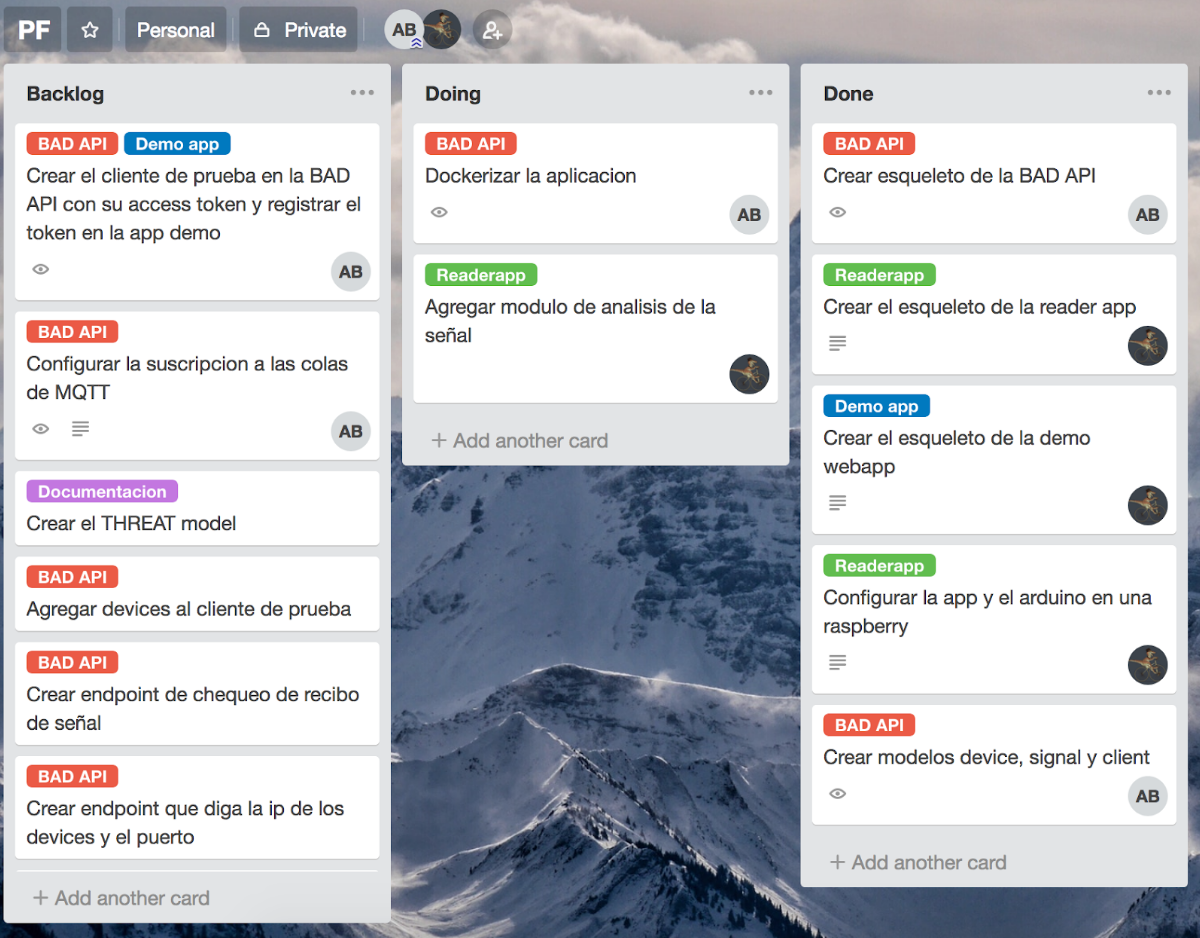
\includegraphics[width=\textwidth]{trelloboard.png}%
    \caption{Board de Trello utilizado}
    \label{fig:trelloboard}
\end{figure}

\paragraph{
Además, utilizamos etiquetas para diferenciar a qué parte del proyecto corresponde cada tarea. Trello cuenta con filtros para poder ver únicamente las tareas de una determinada etiqueta, que facilita la visión de cada proyecto.
}
\paragraph{
En los inicios de los sprints, definimos qué tareas se iban a realizar y se pasaban de “Backlog” a “Doing” y luego a “Done” una vez que se terminaban. Para esto nos era muy útil tener definidas y estimadas las tareas en “Backlog” para luego poder priorizarlas y elegir cual se realizaba en cada sprint según prioridad y dificultad.
}

\begin{figure}[ht]
    \centering
    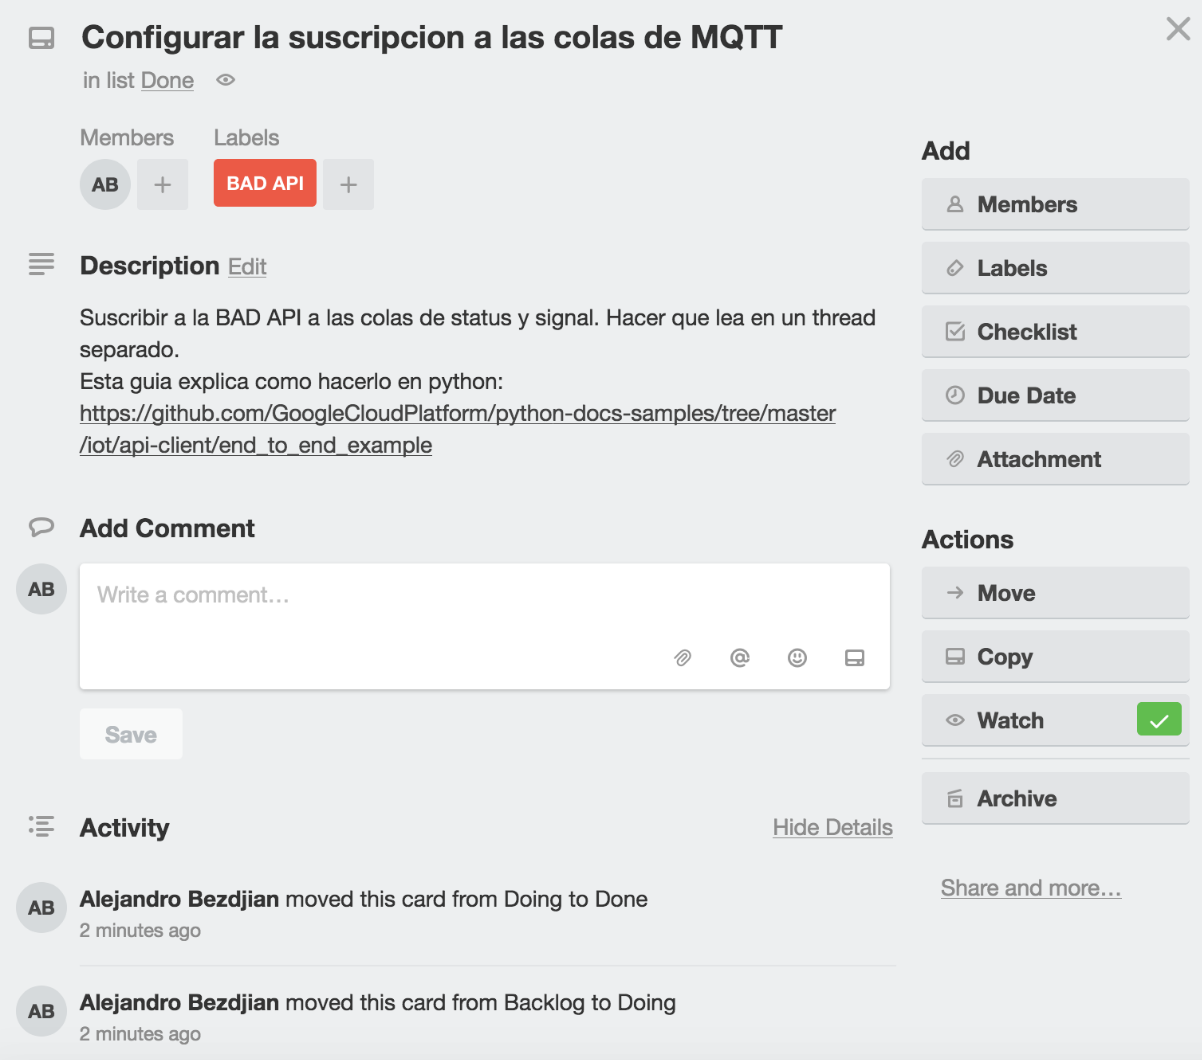
\includegraphics[width=5in]{trellocard.png}%
    \caption{Información de una “card” de Trello}
\end{figure}

\section{Implementación de Referencia}
\paragraph{
Se desarrolló una aplicación de prueba utilizando React en el frontend y Python en el backend para probar las funcionalidades provistas por la BAD API.
}
\paragraph{
Esta aplicación cliente tiene registrados dos dispositivos (Raspberry y laptop) y tiene únicamente las funcionalidades de registro y de login. Los usuarios se registran con un usuario, contraseña y uuid de la señal tomada de la Raspberry.
}
\paragraph{
Dado que la BAD API simplemente compara señales, queda del lado del cliente la decisión de qué hacer con la similitud de las señales y la forma de guardar los UUIDs de las mismas.
}
\paragraph{
Para esta implementación, el cliente guarda en una base de datos PostgreSQL en una tabla “users” el email, la contraseña hasheada con el algoritmo bcrypt y el UUID de la señal obtenida en el registro. Además se optó que el la similitud de las señales debe ser de al menos un 80\% para lograr una autenticación satisfactoria.
}

\begin{figure}[ht]
    \centering
    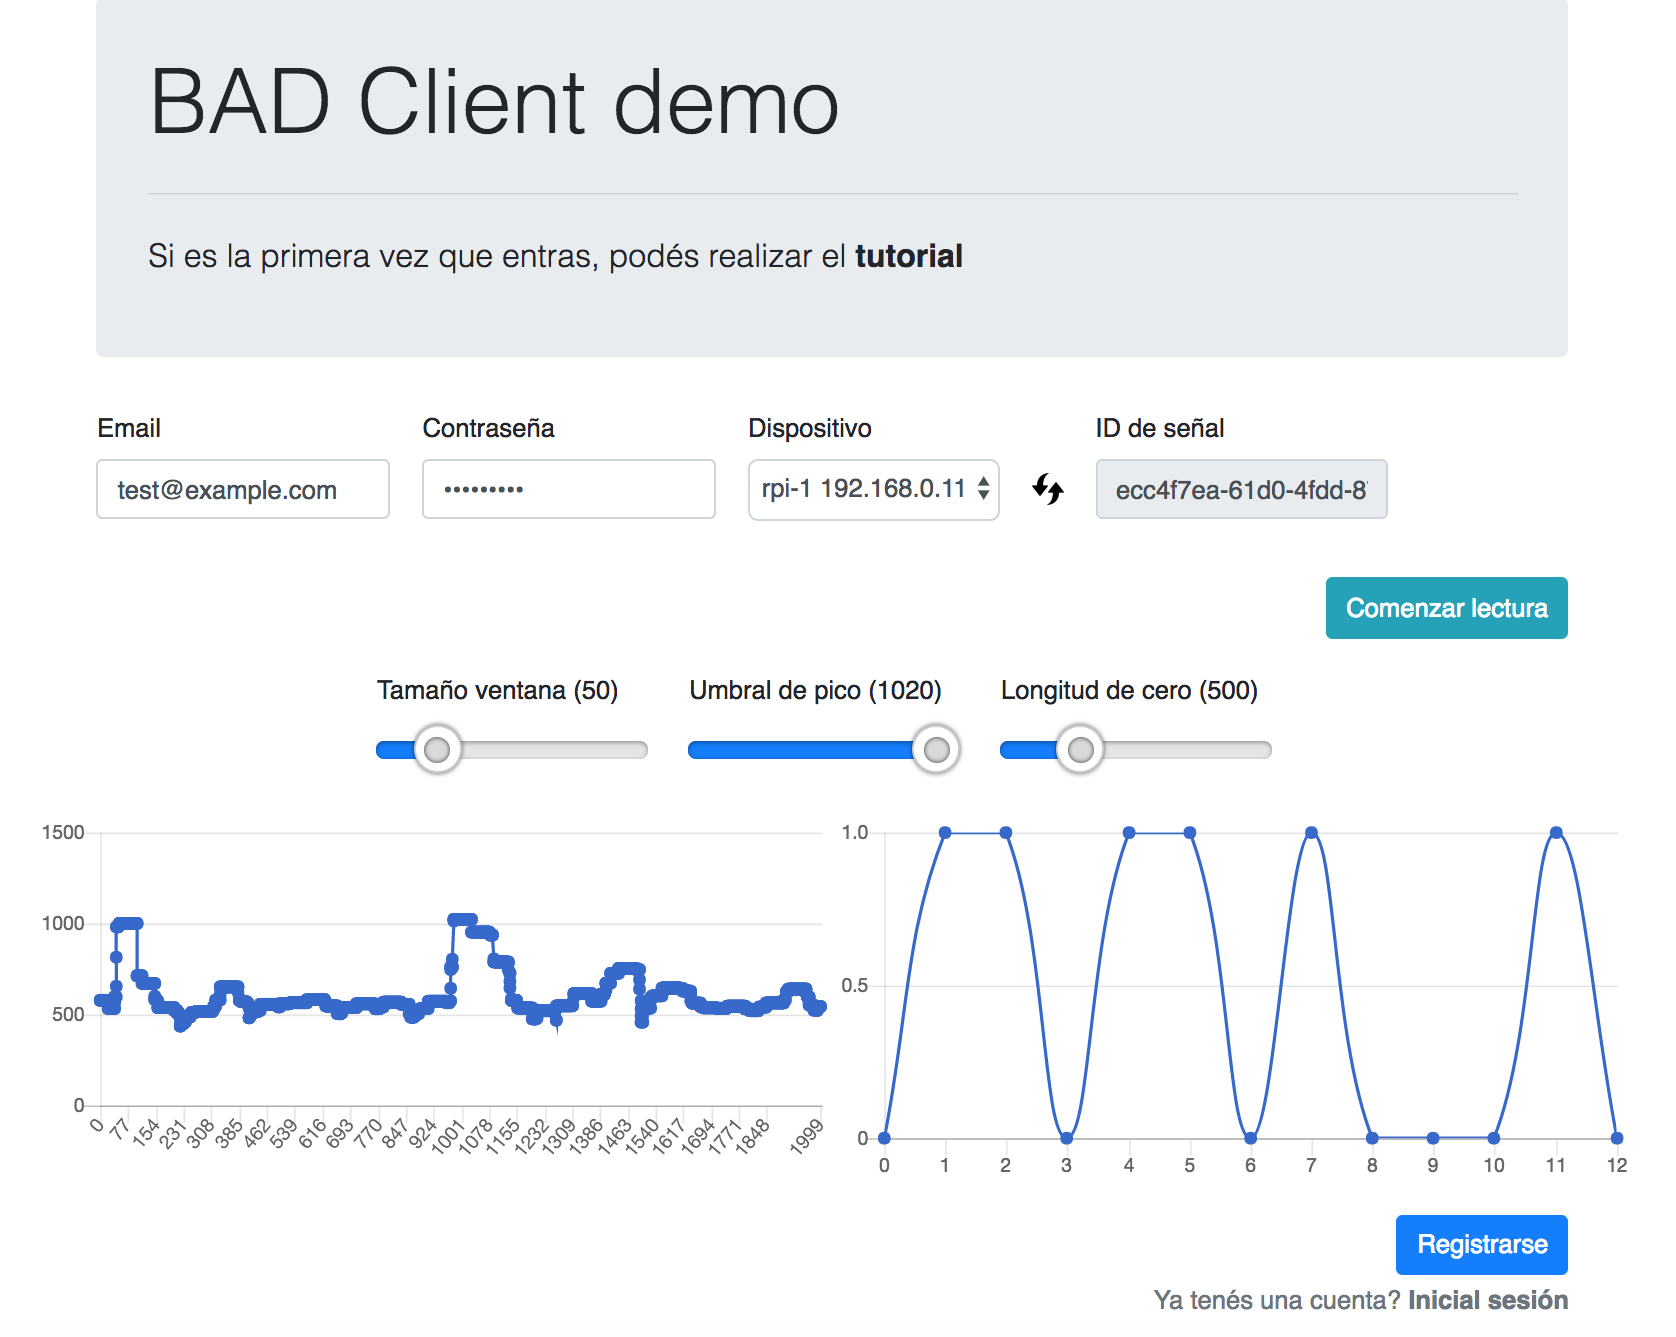
\includegraphics[width=\textwidth]{success_1.png}%
    \caption{Se muestra la señal utilizada para el registro de un usuario de prueba}
    \label{fig:success-1}
\end{figure}

\begin{figure}[ht]
    \centering
    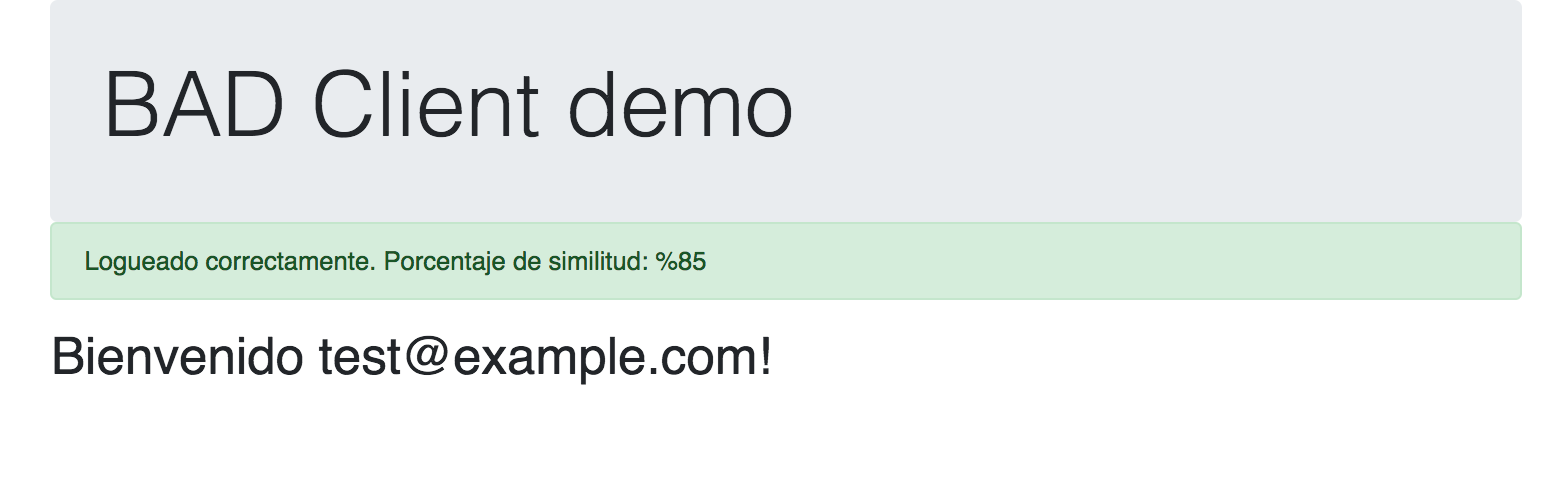
\includegraphics[width=\textwidth]{success_1_result.png}%
    \caption{La similitud de las señales supera el umbral elegido por el cliente y se autentica}
    \label{fig:success-2}
\end{figure}

\begin{figure}[ht]
    \centering
    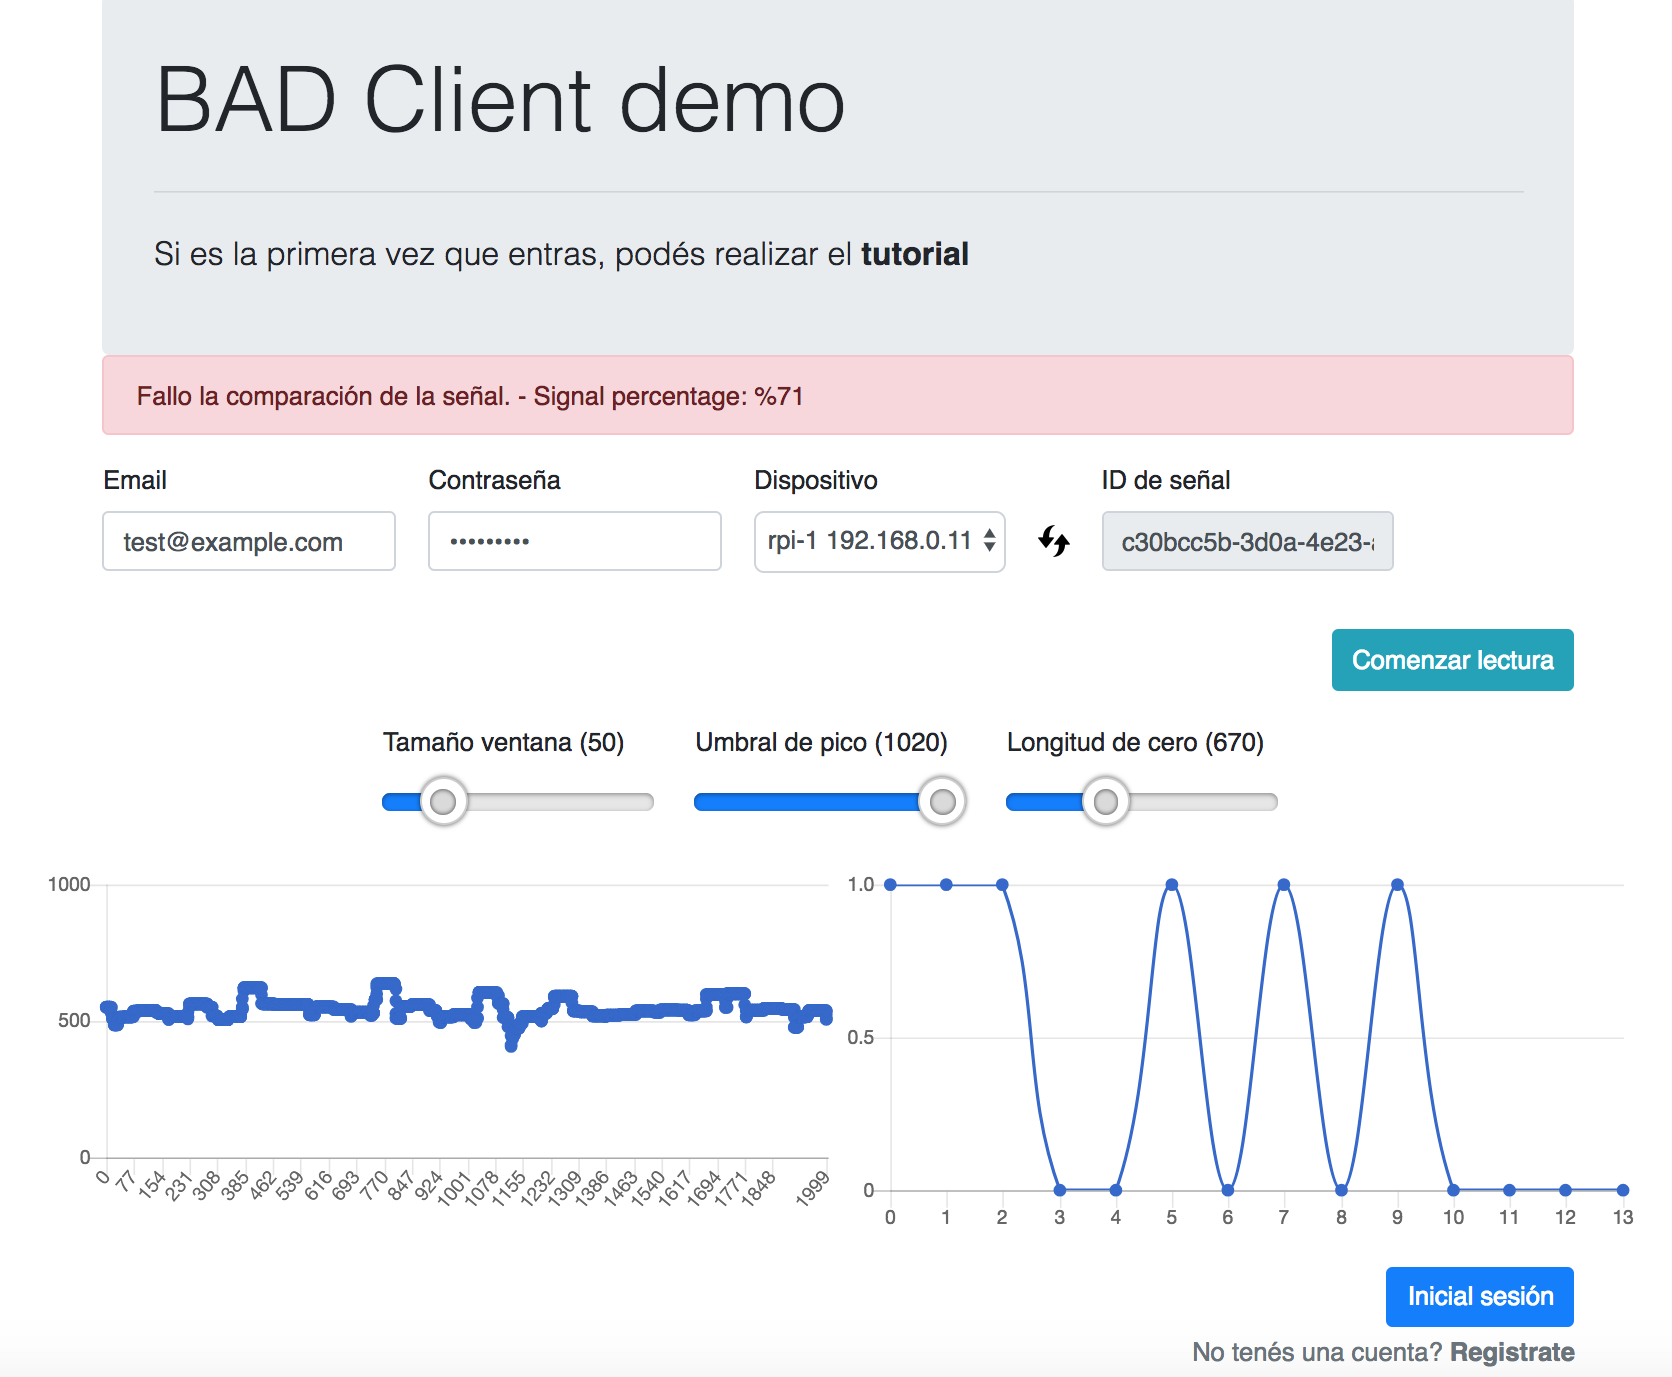
\includegraphics[width=\textwidth]{error_1_res.png}%
    \caption{La autenticación falla porque el porcentaje de similitud de las señales no supera el umbral elegido por el cliente de 80\%}
    \label{fig:error-1}
\end{figure}

\section{Conclusiones}
\paragraph{
El estudio de las señales de EMG, y particularmente EEG, reveló en concordancia con diversos trabajos que son complejas de utilizar para identificar de forma unívoca una persona (acrecentando la diferenciación intra-personal pero disminuyendo la variación inter-personal), lo cual los hace complejos para implementar esquemas de autenticación de manera directa. Sin embargo, con el presente trabajo, demostramos que es posible utilizarlo, para generar un esquema adicional de autenticación que puede servir como segundo factor y que requiere de una participación activa del usuario.
}
\paragraph{
Creemos que la clave para la masificación de este tipo de tecnologías es la implementación de una interfaz genérica por encima de los propios drivers de los dispositivos de lectura de señales, en nuestro caso fue una interfaz HTTPS pero podría ser otra. Esto permite poder adaptar todo tipo de aplicaciones a la utilización de dichas interfaces de manera sencilla, evitando los tipos problemas que se tuvieron con el dispositivo de la marca TrueSense y, además, permite mejorar el dispositivo de captura de la señal sin necesidad de alterar las aplicaciones que lo utilizan.
}
\paragraph{
La tecnología está en un grado de madurez y costo suficientemente bajo como para que se comiencen a utilizar las bioseñales como forma de autenticación de forma obligatoria en servicios que manejan información sensible de los usuarios como los bancarios.
}
\paragraph{
Uno de los problemas más importantes que se presentan cuando se utilizan sistemas de autenticación mediante información intrínseca de las personas, como huellas digitales o iris, es que ante el caso de que se filtre esa información (por un ataque, por ejemplo), los usuarios no pueden cambiarla. Al requerir de una participación activa de los usuarios se puede modificar esta información permitiendo a un usuario recuperar su identidad en el sistema y evitar tener ser dado de baja.
}
\section{Disclaimer}
\paragraph{
Tanto la API como el prototipo no pretenden ser una solución completa y probada sino un punto de partida para eventualmete ofrecer una aplicación comercial. Para evaluar la robustez del sistema es necesario que haya un escrutinio o \textit{penetration testing} realizado por expertos de seguridad. Finalmente para la comercialización es fundamentar conseguir el certificado FIPS de al menos nivel 3 y los certificados para TLS.
}
\section{Trabajo futuro}
\paragraph{
Como trabajo a futuro se planea agregar nuevos dispositivos que utilicen otras funciones biométricas de EMG como EEG (Muse, OpenBCI) para lo cual necesitan de conexión bluetooth LE. Dentro de las posibles mejoras del desarrollo actual se puede utilizar algún dispositivo de lectura de señales de menor tamaño y/o que pueda obtener señales con mayor velocidad y/o fidelidad. Estos últimos puntos son útiles para aumentar la aceptación psicológica de los usuarios.
}
\paragraph{
Una aplicación relacionada sería la utilización de esta tecnología para identificar a la persona en base a las señales de EMG en el momento en que realiza una firma sobre un papel, su firma de puño y letra.  Este esquema obtendría un fingerprint de las señales de EMG similares a lo realizado en este trabajo, con el agregado del componente activo que agregue un eje más de verificación y que permite la actualización de la información complementaria en el caso de que la misma sea comprometida.  Además generaría un beneficio en cuánto a la aceptación de la misma ya que la firma de puño y letra es un mecanismo natural para proveer de una autenticidad a documentos legales y burocráticos. En caso de funcionar, podría transformarse en una forma muy útil de firmar pagos electrónicos.
}

\paragraph{
Este tipo de soluciones tiene aplicaciones directas sobre la accesibilidad, para personas con discapacidad, como por ejemplo en el trabajo realizado en \cite{haberman2016} donde se realizó un estudio específico de los biopotenciales de EMG en una aplicación para personas con discapacidades motoras utilizando un protocolo similar al ofrecido por la BAD API. En el mismo se implementa un prototipo de dispositivo de ayuda tipo switch que emite pulsos binarios generados a partir de señales EMG. Un posible trabajo futuro podría ser realizar una interfaz genérica que permita comunicar este tipo de dispositivos con aplicaciones web o de escritorio de forma tal que sea más fácil la incorporación de nuevos dispositivos.
}

\paragraph{
Además de los usos actuales de EMG y EEG, otros usos innovadores de estas señales podrían ser en la industria automotriz (por ejemplo para que los autos solo puedan ser abiertos y encendidos por ciertas personas, para activar el manejo autónomo o incluso para manejar) o el manejo de drones.
}



\clearpage
\nocite{opinnovationswebsite}
\nocite{charbit2017}
\nocite{bressert2012}
\nocite{angkoon2009}
\nocite{oliphant2015}
\nocite{langtangen2016}
\nocite{hassanien2015}
\nocite{moonwon2016}
\nocite{sharma2016}
\nocite{trewin}
\nocite{chowdhury2013}
\nocite{siqueira2015}
\nocite{samsung2016}
\nocite{raez2006}
\nocite{esparza2017}
\nocite{sanei2007}
\nocite{haberman2016}

\printbibliography[heading=bibintoc,title={Bibliografía}]
\end{document}
